
\section{2 lepton training for high $e_T^{miss}$ and invariant mass search}\label{sec:2lep}

The 3 lepton + $e_T^{miss}$ dataset has fewer events, and thus allows for less training of the neural networks. 
Thus, the 2 lepton + $e_T^{miss}$ dataset was tried as well. The event selection was done choosing at least 
2 leptons, meaning that the RMM signatures of some events will look similar to the RMM signatures of 
the 3 lepton + $e_T^{miss}$ dataset. A consequence of this is that the signal samples for the 3 lepton case 
works well for testing the autoencoders trained on the 2 lepton + $e_T^{miss}$ dataset. The two autoencoders will be tested on three of the 
four metrics used for the 3 lepton + $e_T^{miss}$ case. 
\begin{itemize}
    \item Low reconstruction error on SM MC
    \item Background to signal ratio in $e_T^{miss}$ signal region
    \item Significance search in $e_T^{miss}$ signal region
\end{itemize}

\subsubsection*{Regular autoencoder performance}
Below are some results from training on the 2 lepton case with the regular autoencoder, using the same two SUSY signals as test cases. 

\begin{figure}[h!]
    \centering
    \begin{subfigure}{.49\textwidth}
        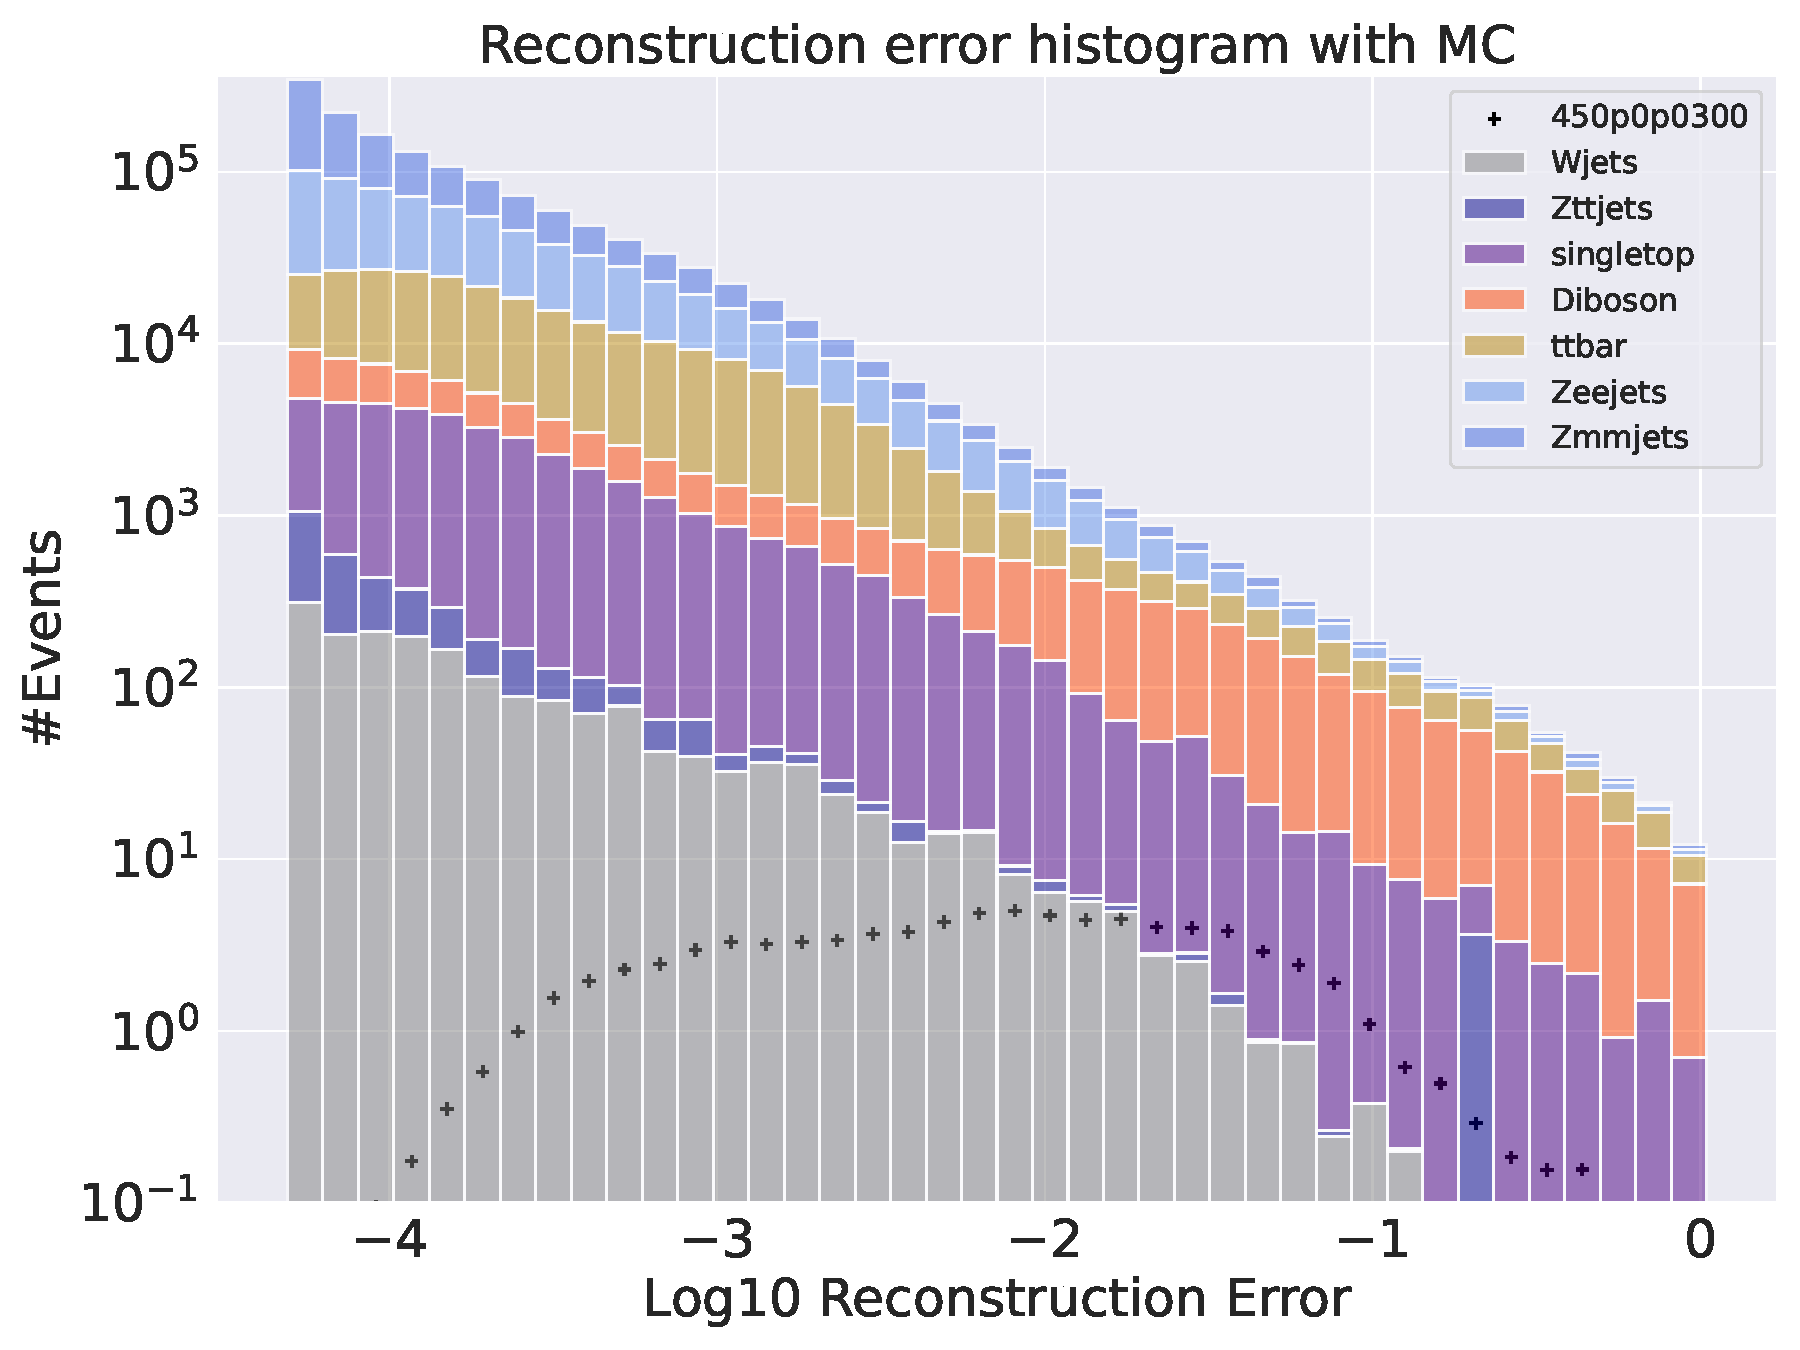
\includegraphics[width=\textwidth]{Figures/AE_testing/small/2lep/b_data_recon_big_rm3_feats_sig_450p0p0300_.pdf}
        \caption{ }
        \label{fig:AE_2lep_big_450}
    \end{subfigure}
    \hfill
    \begin{subfigure}{.49\textwidth}
        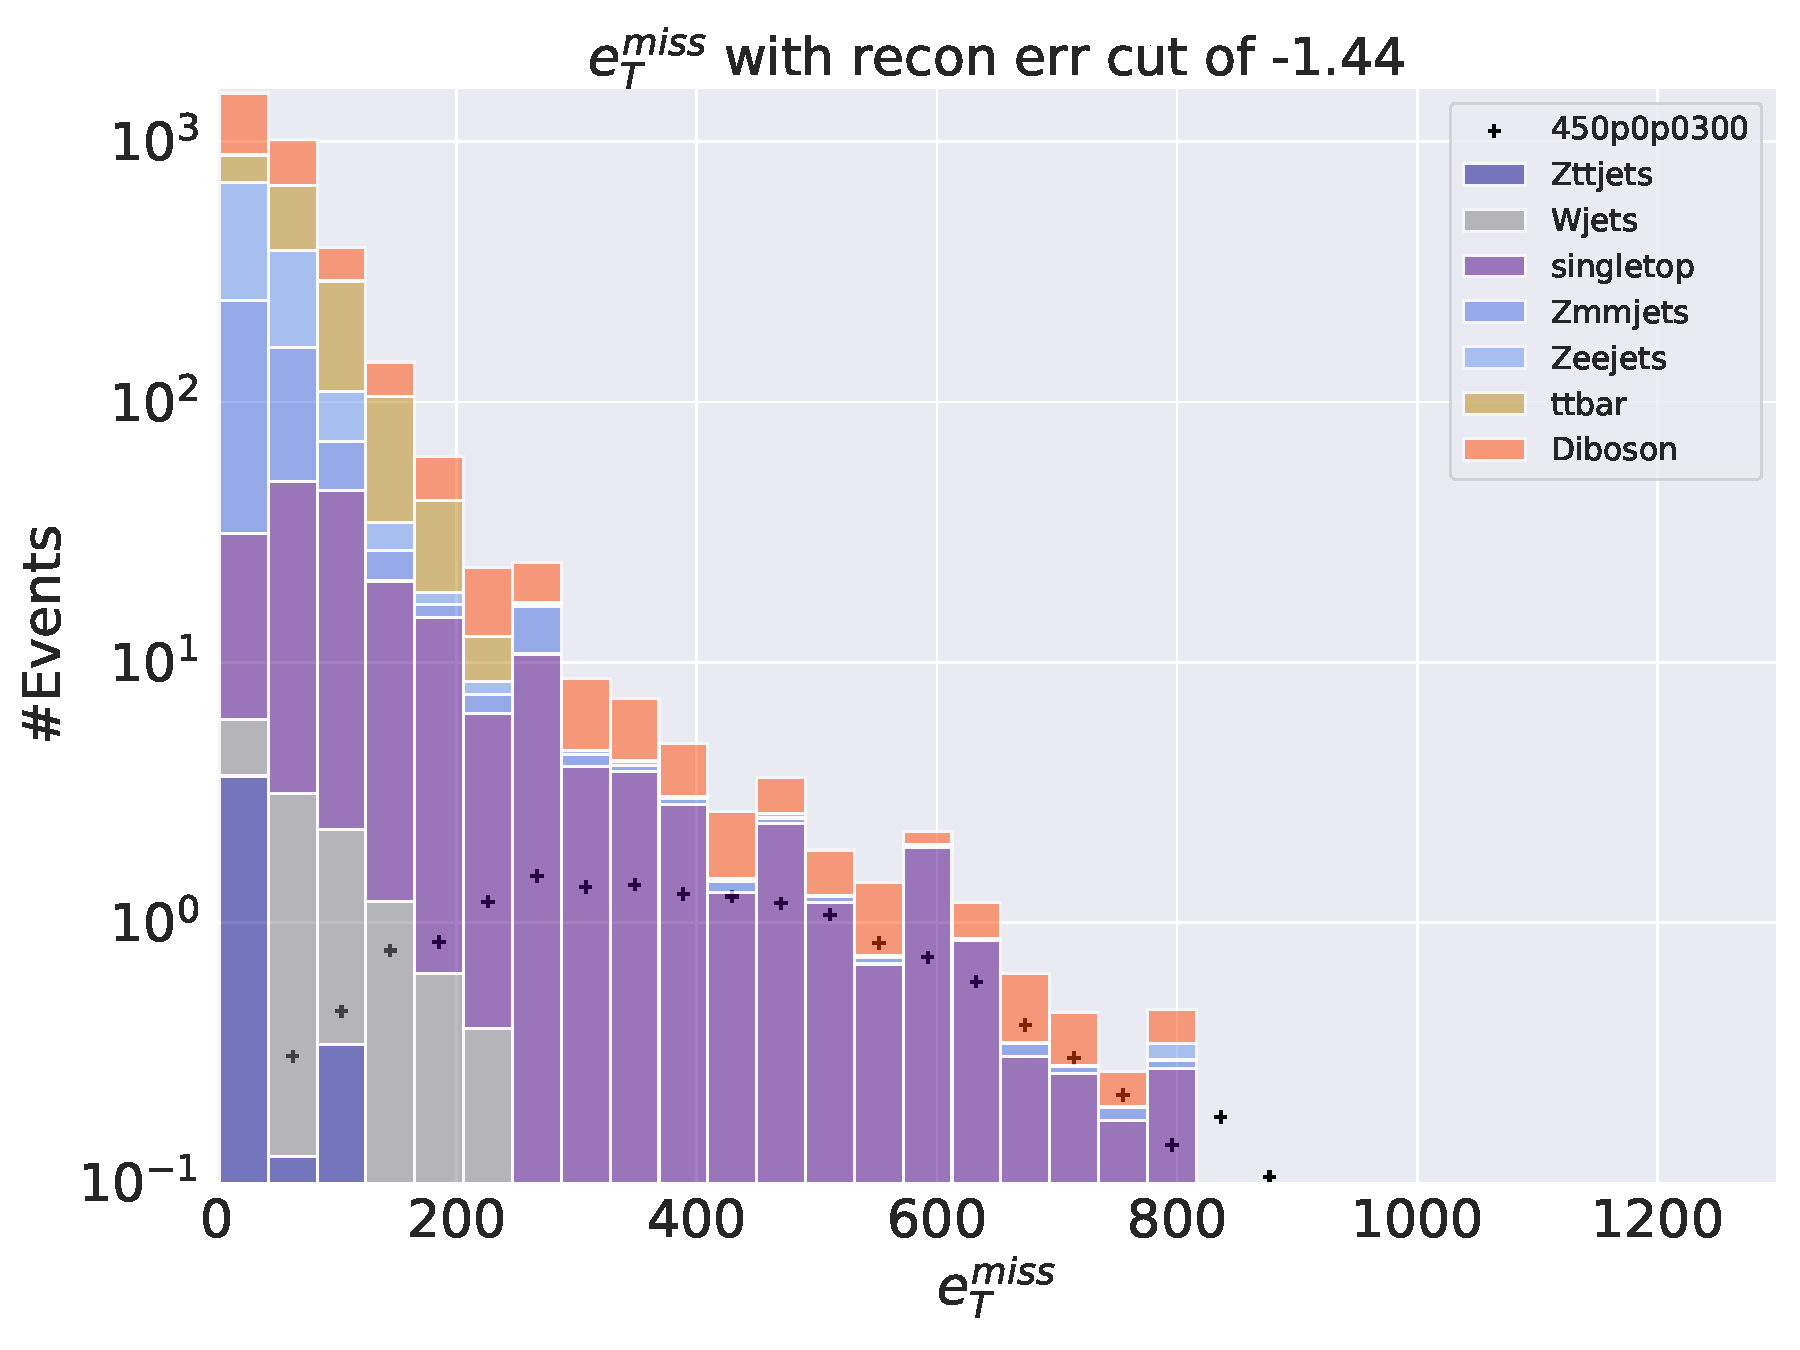
\includegraphics[width=\textwidth]{Figures/AE_testing/big/2lep/b_data_recon_big_rm3_feats_sig_450p0p0300_recon_errcut_-1.44.pdf}
        \caption{}
        \label{fig:AE_2lep_big_etmiss_450}
    \end{subfigure}
    \hfill 
    \begin{subfigure}{.49\textwidth}
        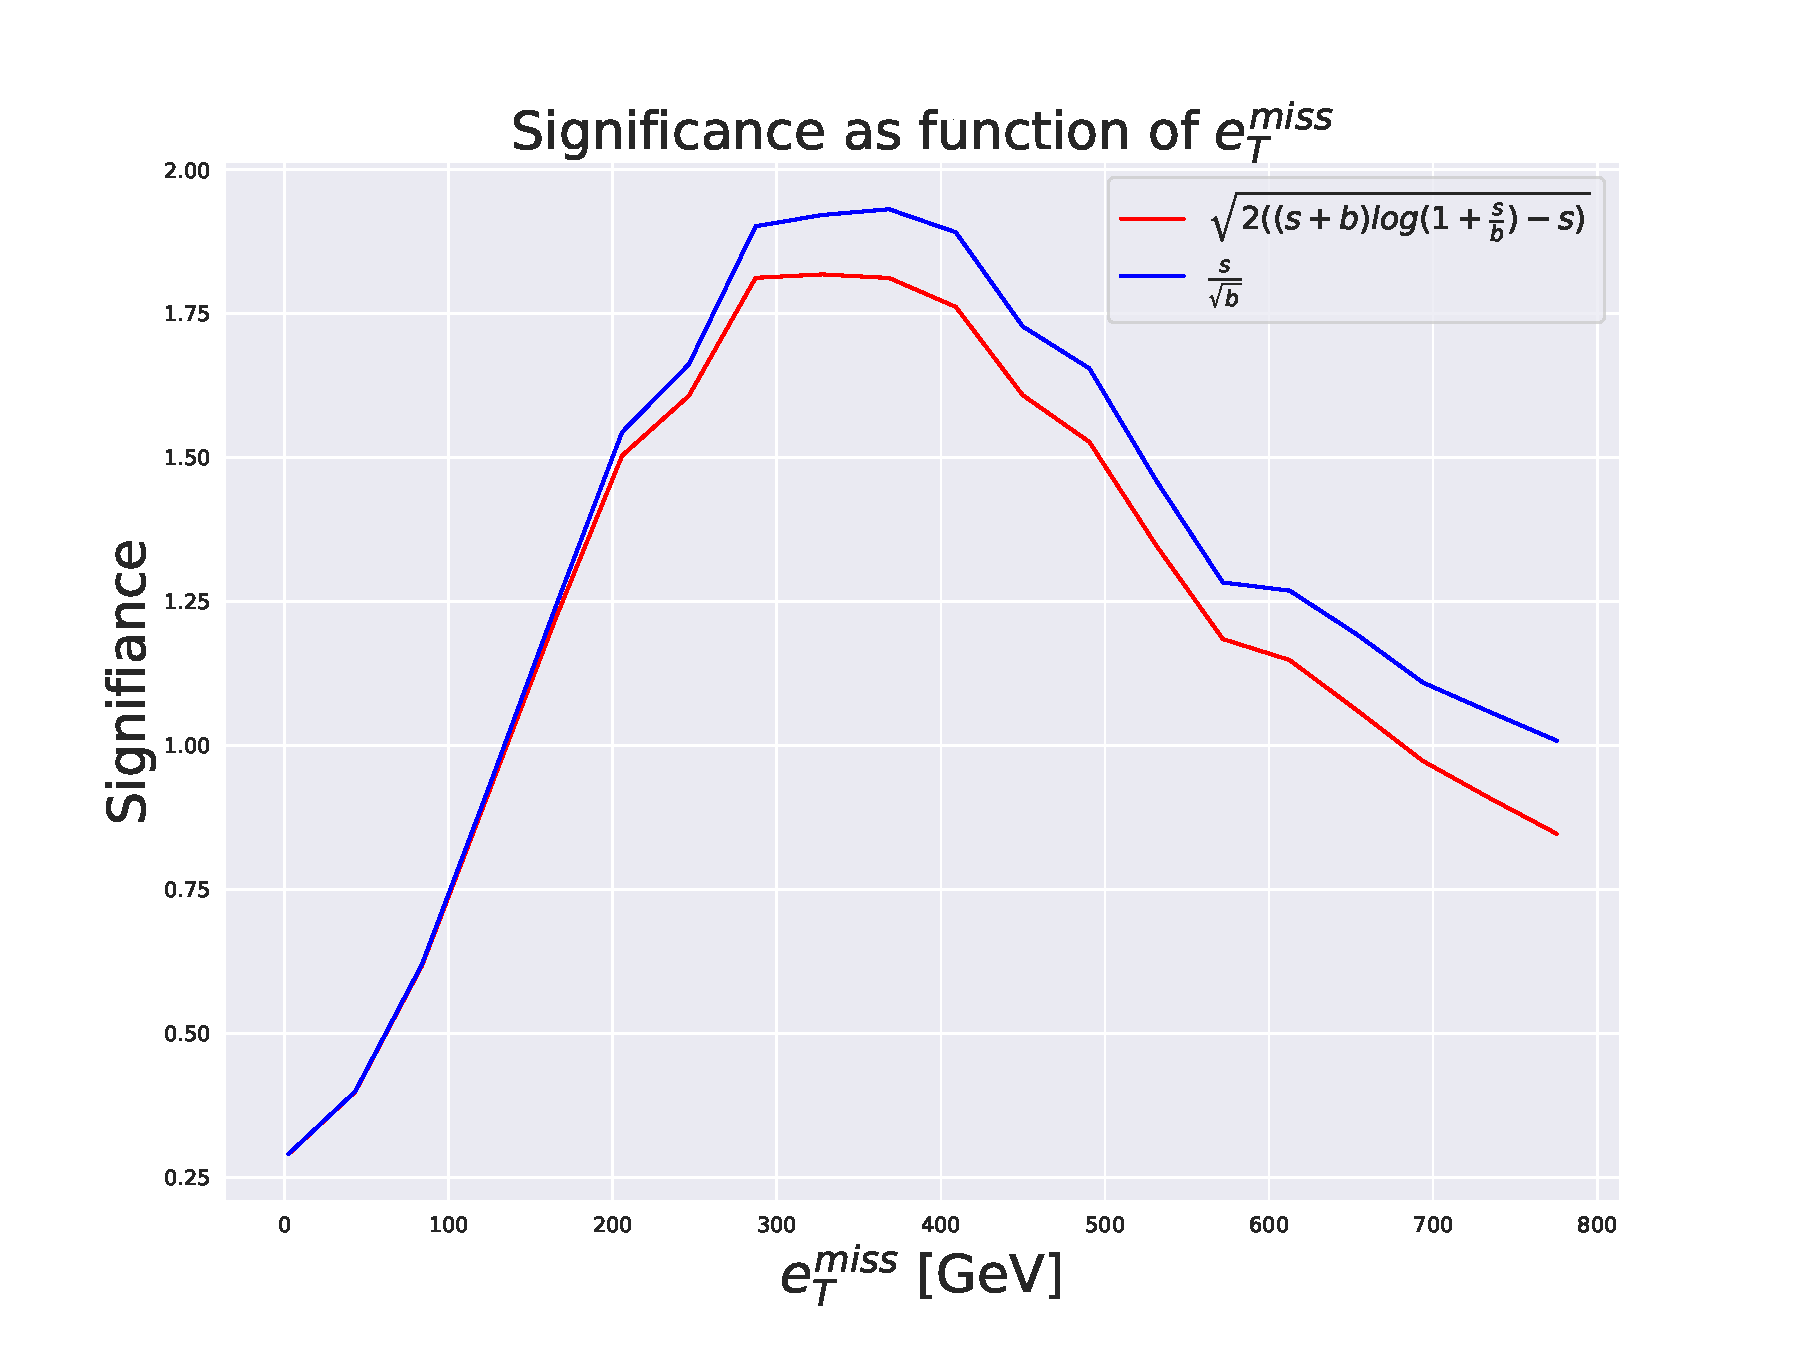
\includegraphics[width=\textwidth]{Figures/AE_testing/big/2lep/significance_etmiss_450p0p0300_-1.4360553938127363.pdf}
        \caption{}
        \label{fig:AE_2lep_big_signi_450}
    \end{subfigure}
    \hfill      
    \caption[2lep deep network | $450p300$ | AE]{Reconstruction error (a), $e_T^{miss}$ signal region (b) and significance as function of 
    $e_T^{miss}$ (c) for the deep regular autoencoder using SUSY $450p300$. 
    (a) shows the reconstruction error distribution for the SM MC and the SUSY signal. 
    The autoencoder produces a slope-like shape that is highly shifted to the lower end of the reconstruction error range
for the background. The signal is more evenly spread out along the x-axis. The peaks of the two distributions are totally separated
with two orders of magnitude in reconstruction error. (b) shows the $e_T^{miss}$
T distribution for the SM MC and the SUSY signal in the signal region. The signal region is made using a cut around
$10^{-1.44}$. Most of the background is removed, and the peaks of the SM MC and signal distributions are
somewhat separated. (c) shows the significance as function of $e_T^{miss}$. The peak is put 
around a cut of about 380 GeV in the $e_T^{miss}$, with a significance of around $1.85$.}
    \label{fig:AE_2lep_big_rec_sig_signi_450}
\end{figure}



\begin{figure}[h!]
    \centering
    \begin{subfigure}{.49\textwidth}
        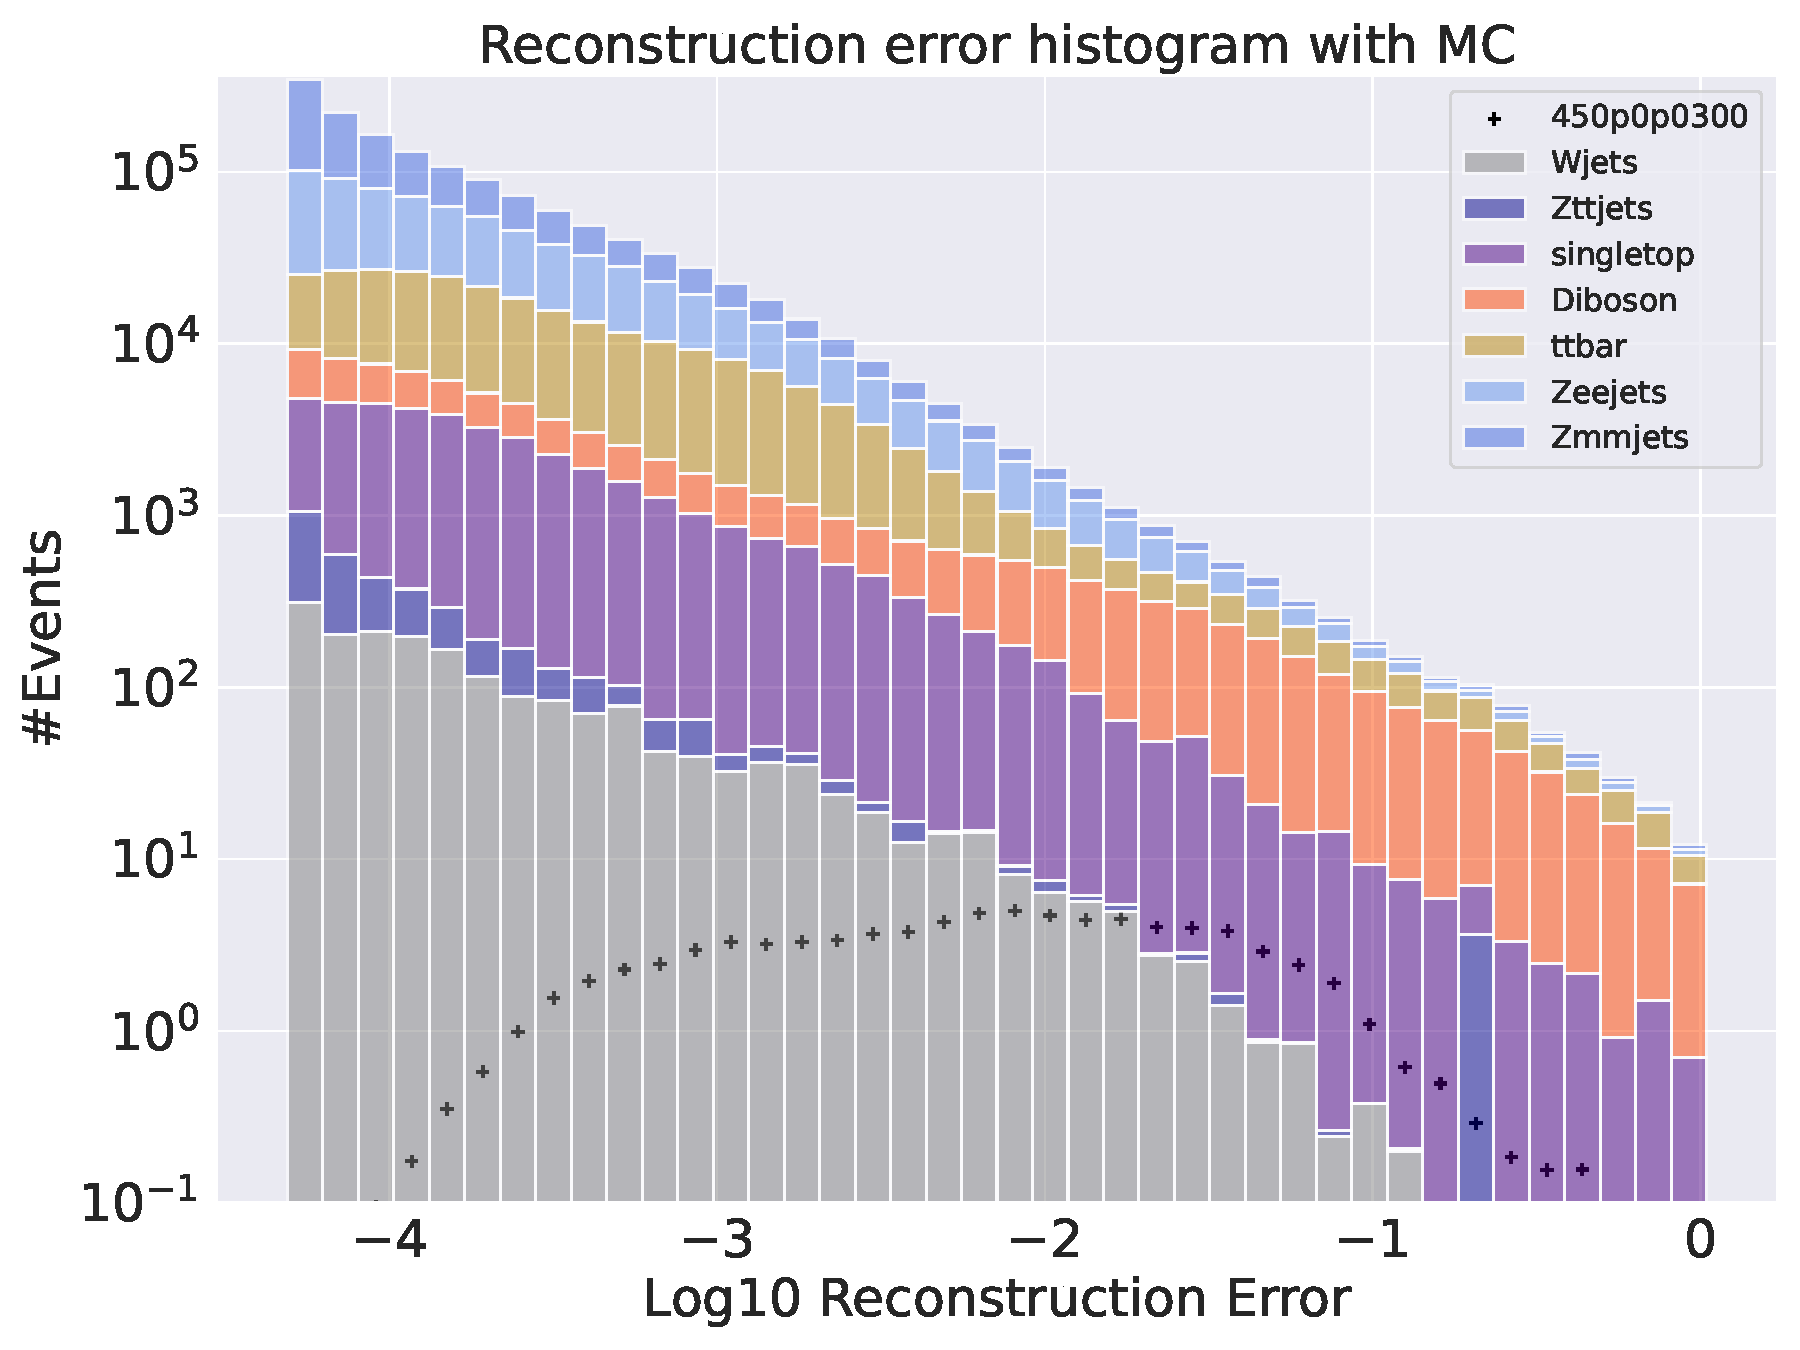
\includegraphics[width=\textwidth]{Figures/AE_testing/small/2lep/b_data_recon_big_rm3_feats_sig_450p0p0300_.pdf}
        \caption{ }
        \label{fig:AE_2lep_small_450}
    \end{subfigure}
    \hfill
    \begin{subfigure}{.49\textwidth}
        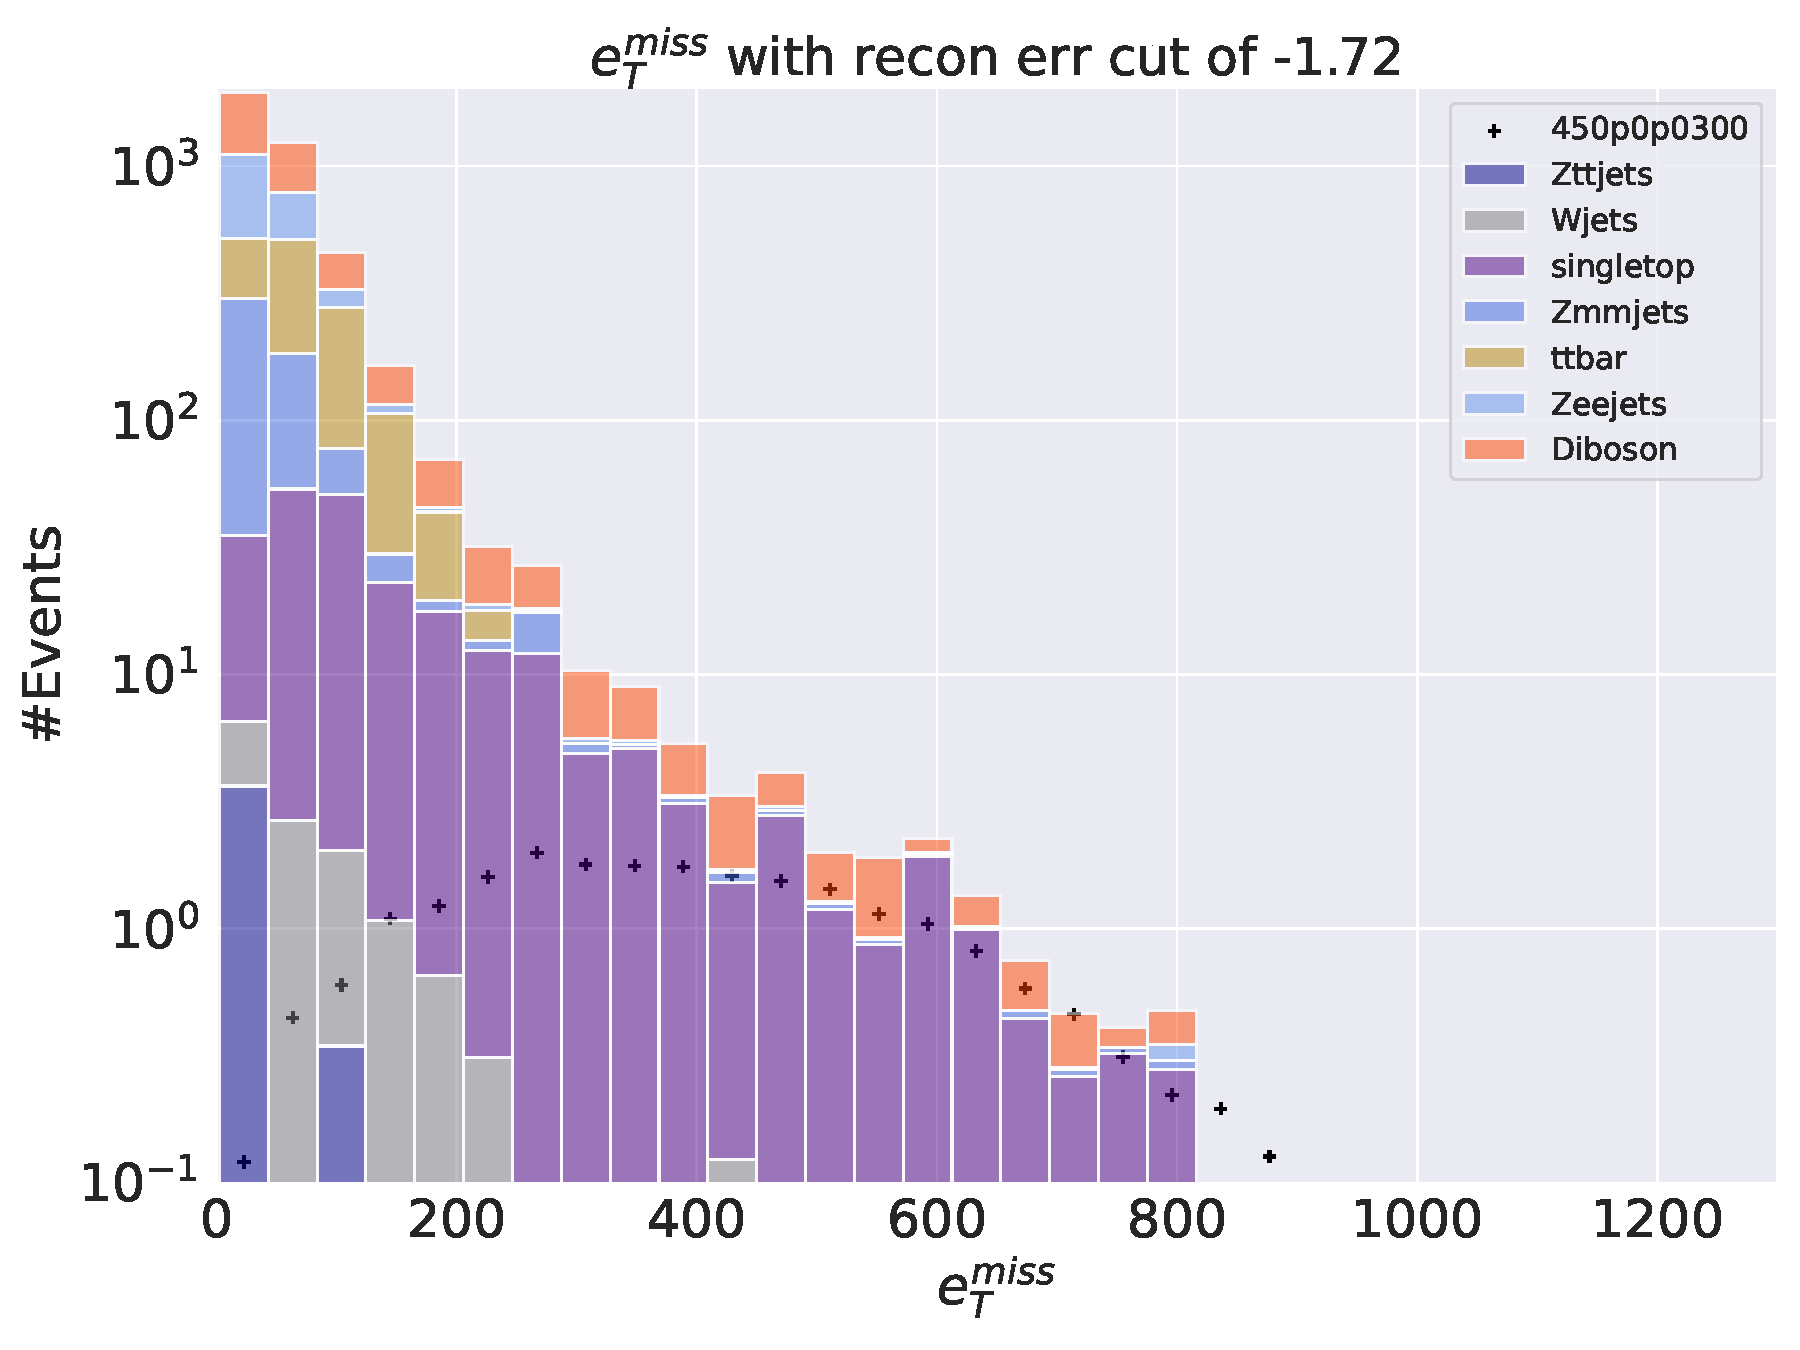
\includegraphics[width=\textwidth]{Figures/AE_testing/small/2lep/b_data_recon_big_rm3_feats_sig_450p0p0300_recon_errcut_-1.72.pdf}
        \caption{}
        \label{fig:AE_2lep_small_etmiss_450}
    \end{subfigure}
    \hfill  
    \begin{subfigure}{.49\textwidth}
        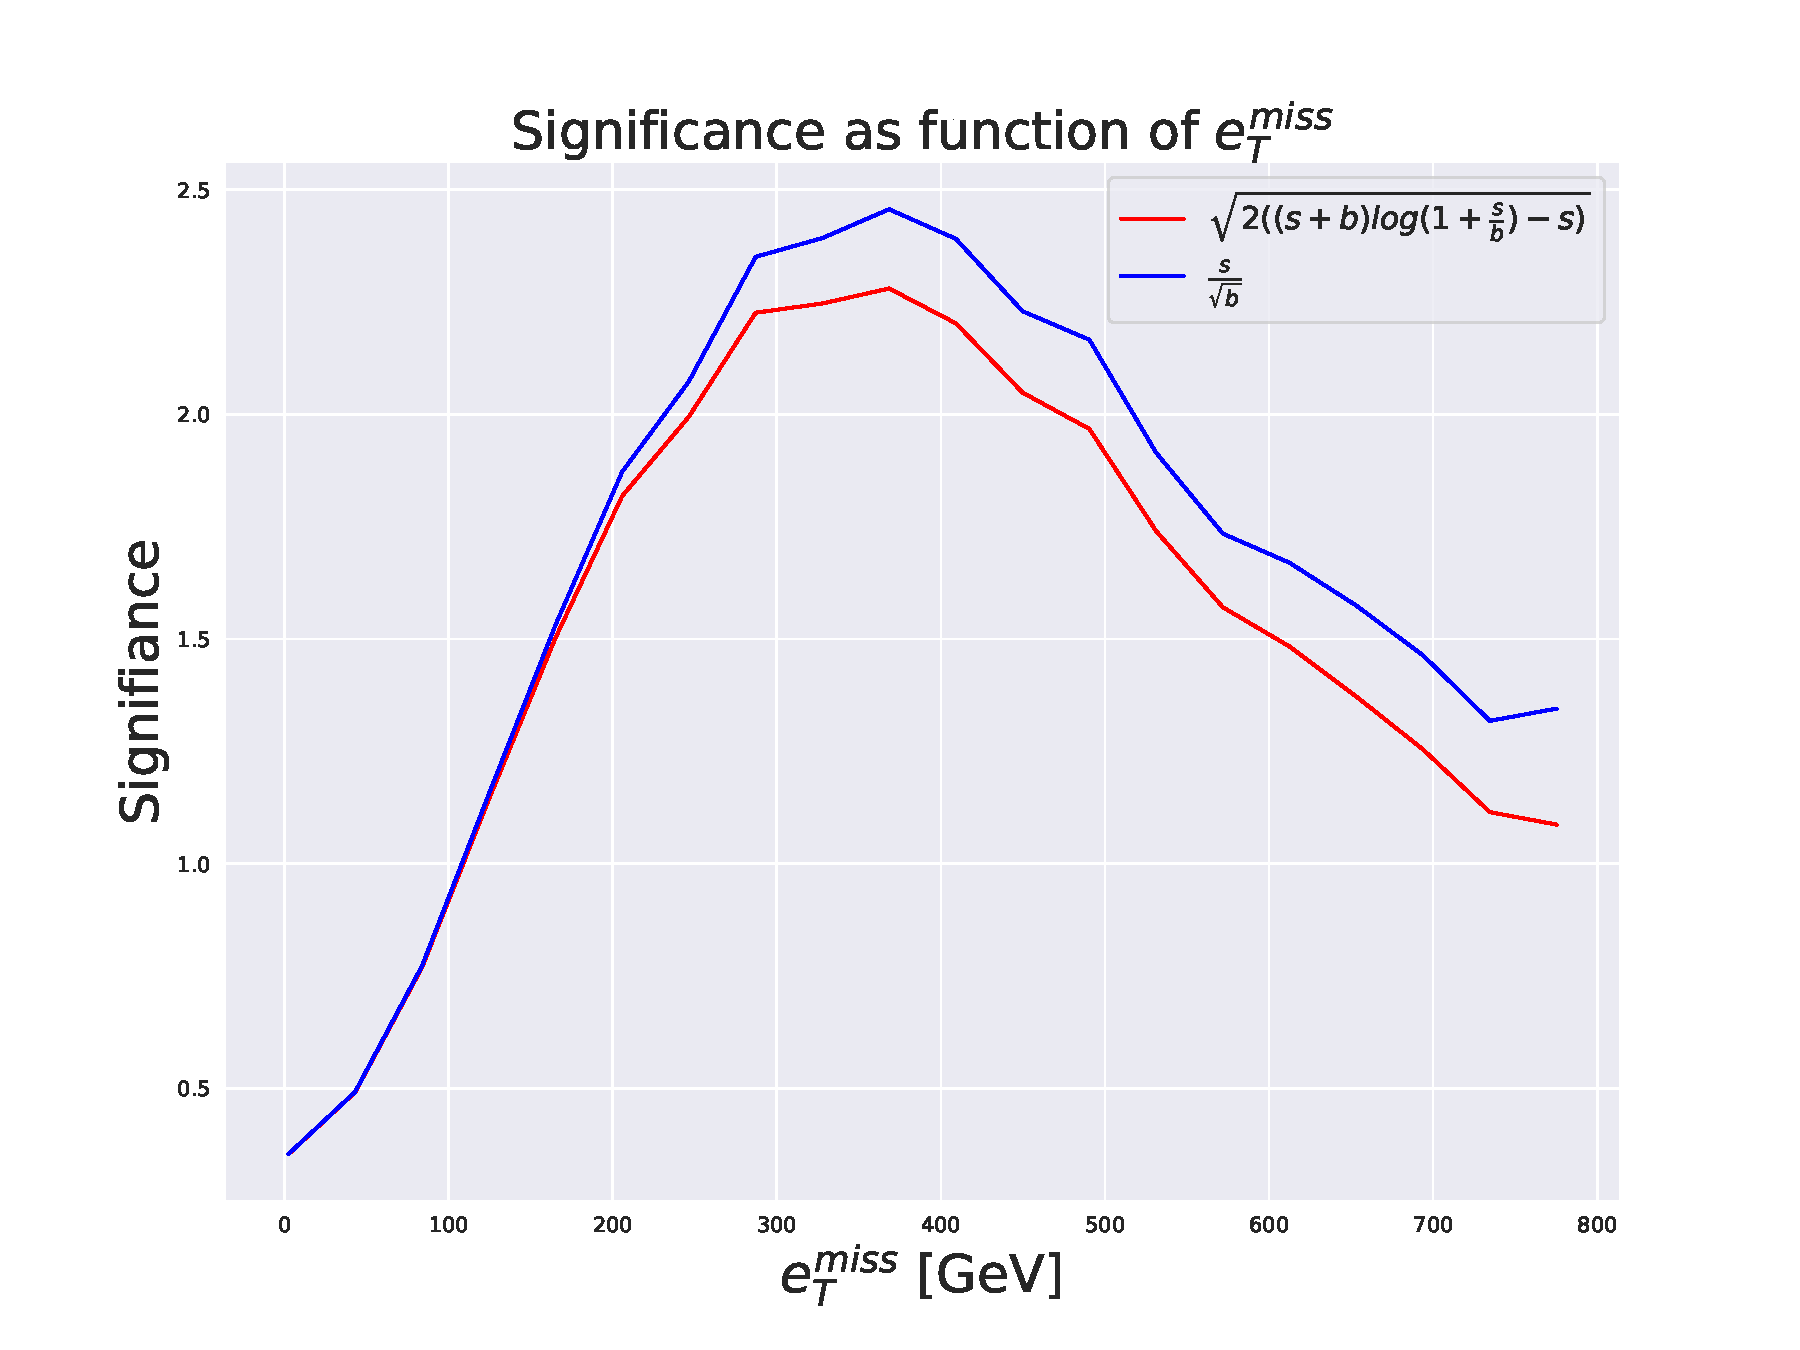
\includegraphics[width=\textwidth]{Figures/AE_testing/small/2lep/significance_etmiss_450p0p0300_-1.7167506533614734.pdf}
        \caption{}
        \label{fig:AE_2lep_small_signi_450}
    \end{subfigure}
    \hfill      
    \caption[2lep shallow network | $450p300$ | AE]{Reconstruction error (a), $e_T^{miss}$ signal region (b) and significance as function of 
    $e_T^{miss}$ (c) for the deep regular autoencoder using SUSY $450p300$. 
    (a) shows the reconstruction error distribution for the SM MC and the SUSY signal. 
    The autoencoder produces a slope-like shape that is highly shifted to the lower end of the reconstruction error range
for the background. The signal is more evenly spread out along the x-axis. The peaks of the two distributions are totally separated
with two orders of magnitude in reconstruction error. (b) shows the $e_T^{miss}$
T distribution for the SM MC and the SUSY signal in the signal region. The signal region is made using a cut around
$10^{-1.72}$. Most of the background is removed, and the peaks of the SM MC and signal distributions are
somewhat separated. (c) shows the significance as function of $e_T^{miss}$. The peak is put 
around a cut of about 380 GeV in the $e_T^{miss}$, with a significance of around $2.4$.}
    \label{fig:AE_2lep_small_rec_sig_signi_450}
\end{figure}


\begin{figure}[h!]
    \centering
    \begin{subfigure}{.49\textwidth}
        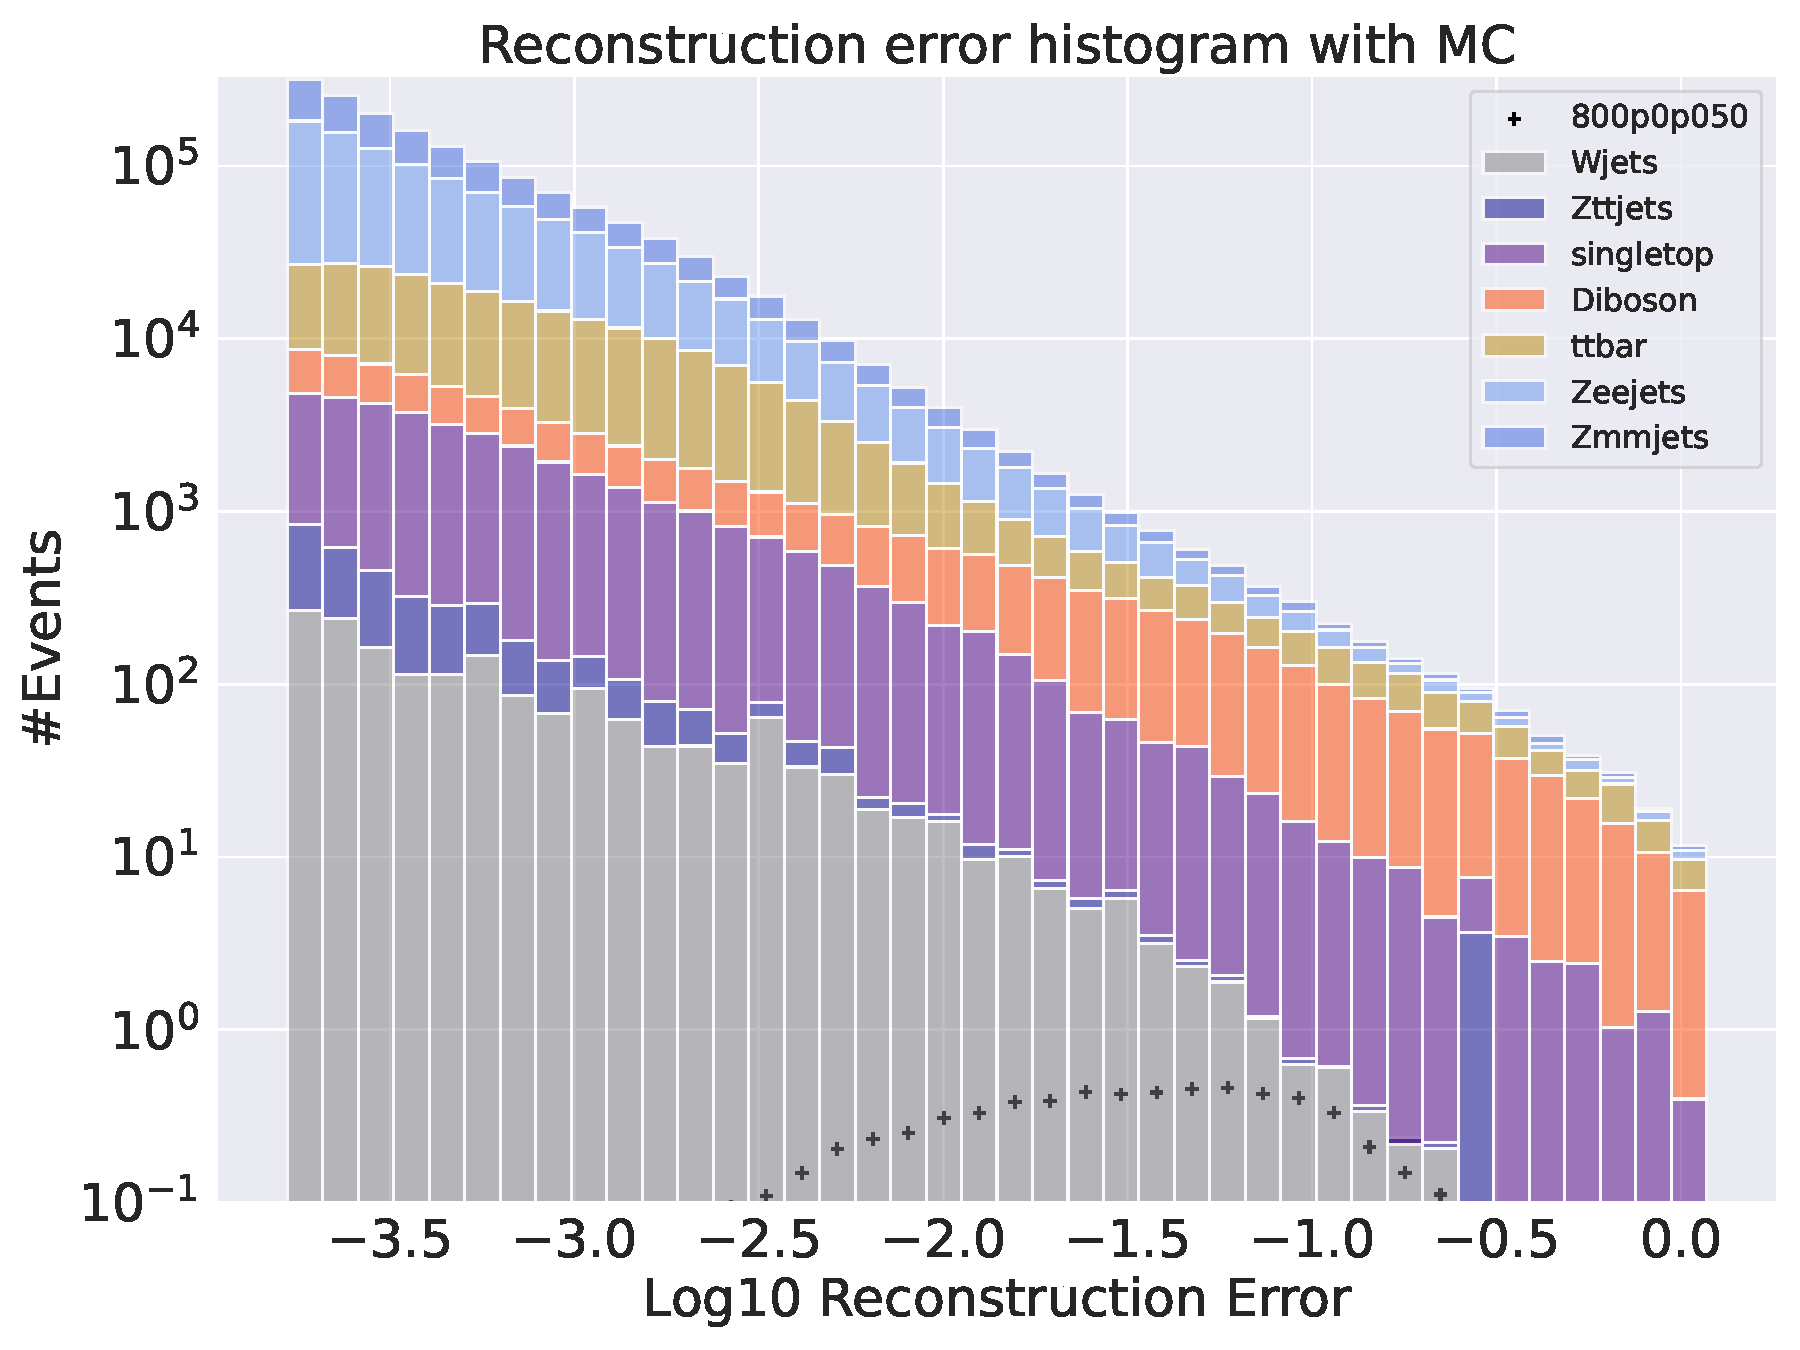
\includegraphics[width=\textwidth]{Figures/AE_testing/big/2lep/b_data_recon_big_rm3_feats_sig_800p0p050_.pdf}
        \caption{ }
        \label{fig:AE_2lep_big_800}
    \end{subfigure}
    \hfill
    \begin{subfigure}{.49\textwidth}
        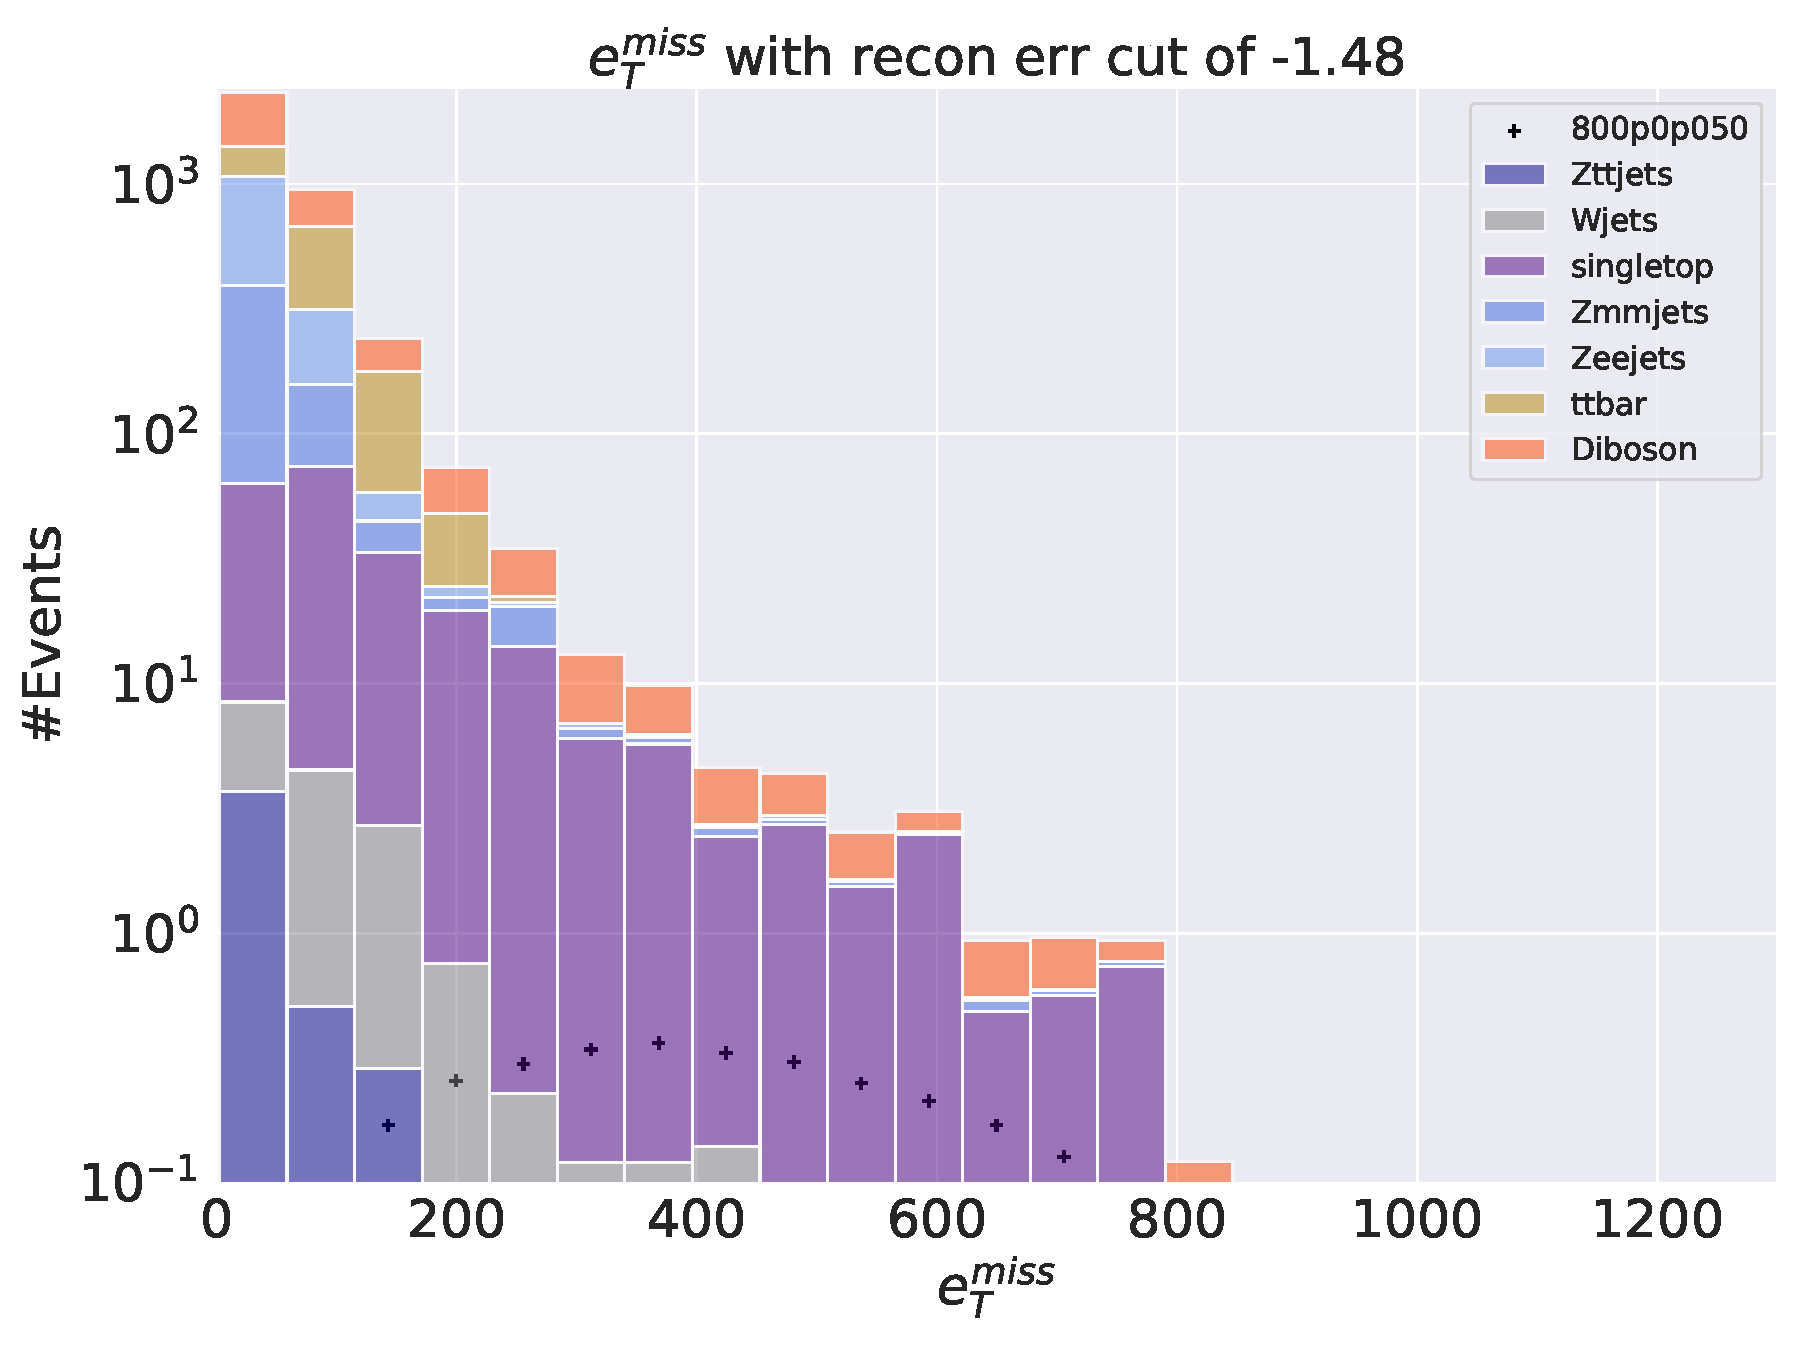
\includegraphics[width=\textwidth]{Figures/AE_testing/big/2lep/b_data_recon_big_rm3_feats_sig_800p0p050_recon_errcut_-1.48.pdf}
        \caption{}
        \label{fig:AE_2lep_big_etmiss_800}
    \end{subfigure}
    \hfill
      
    \begin{subfigure}{.49\textwidth}
        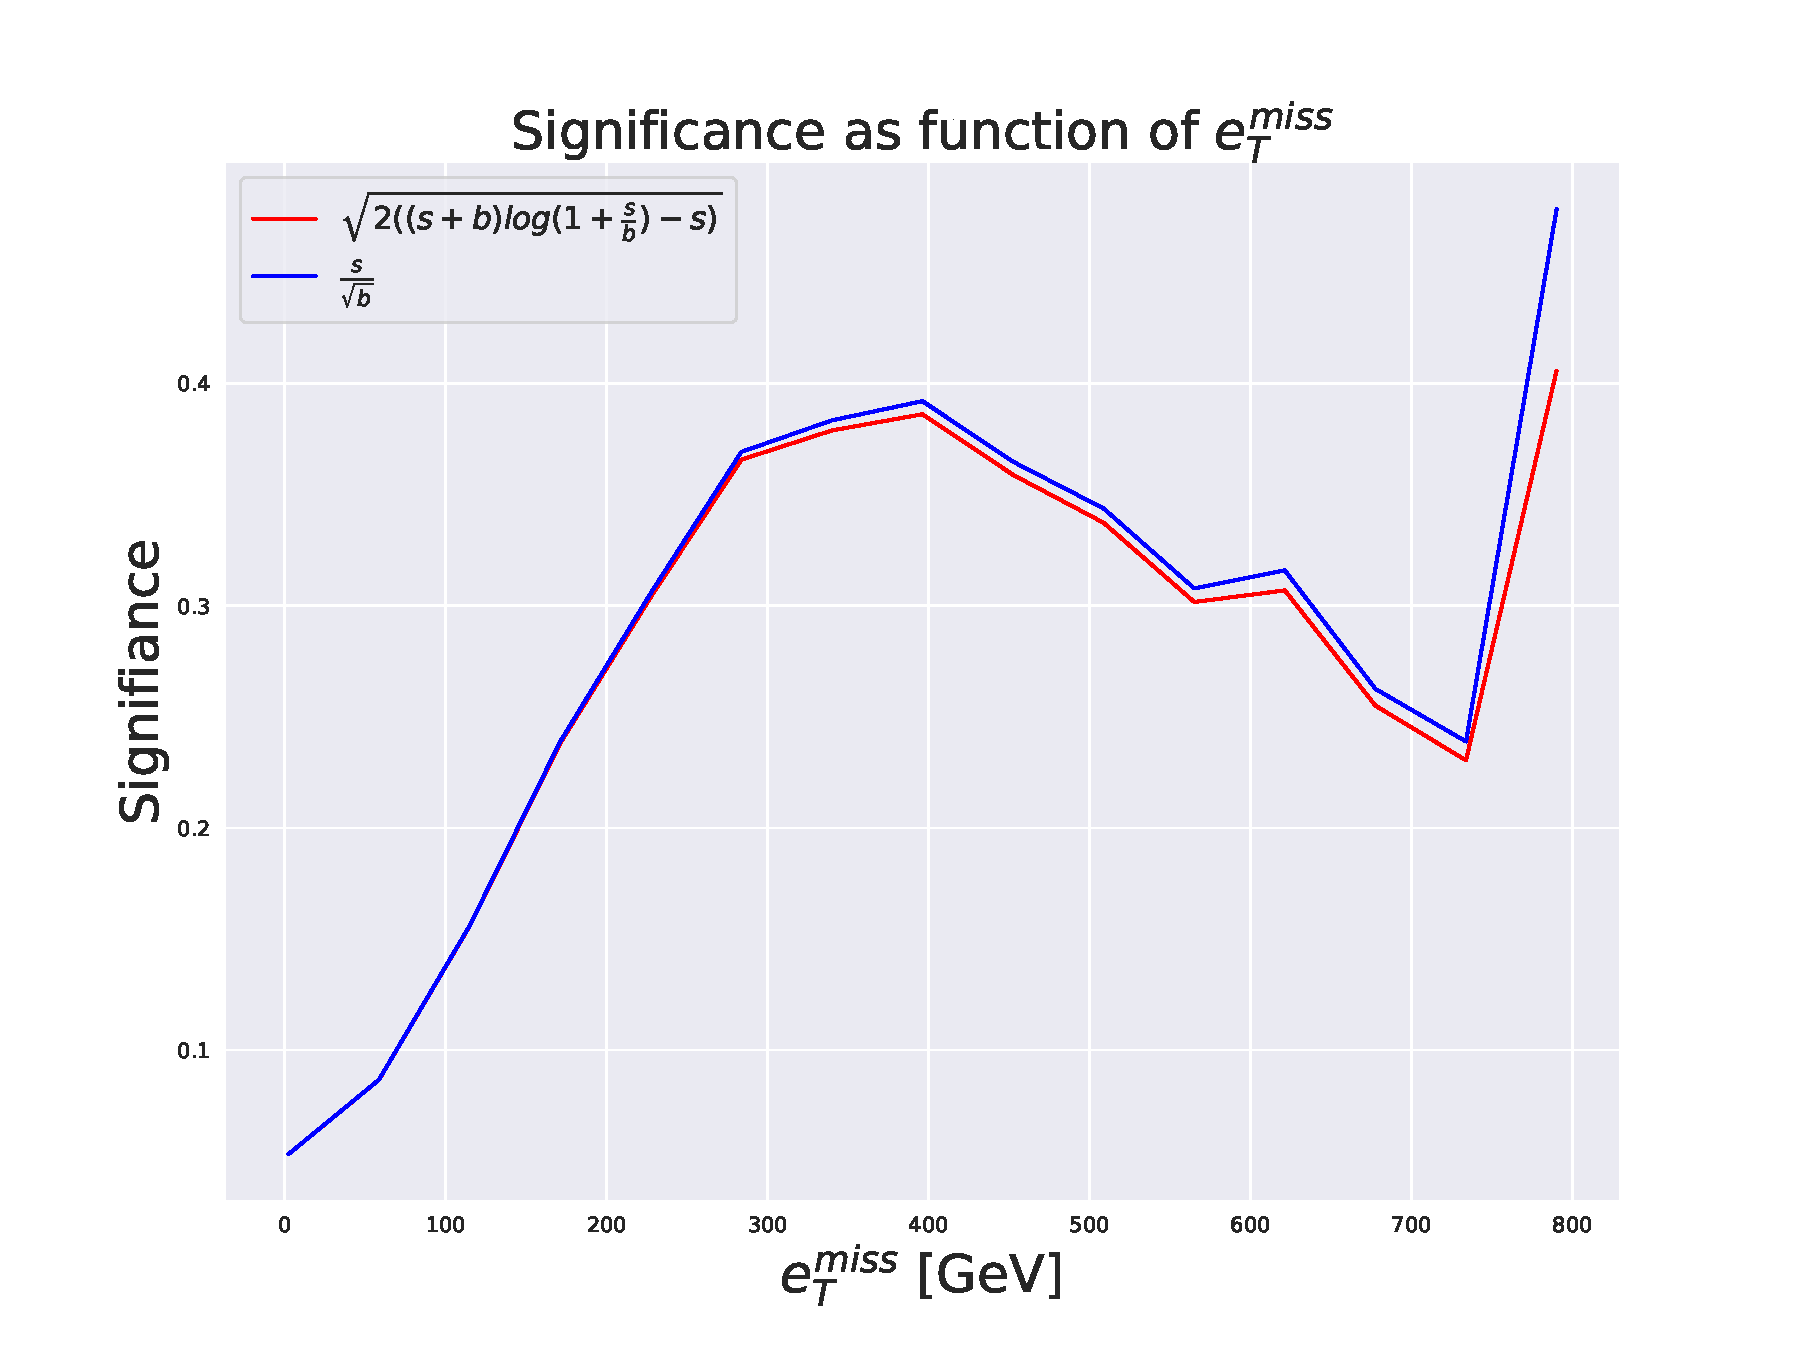
\includegraphics[width=\textwidth]{Figures/AE_testing/big/2lep/significance_etmiss_800p0p050_-1.4833711230716062.pdf}
        \caption{}
        \label{fig:AE_2lep_big_signi_800}
    \end{subfigure}
    \hfill      
    \caption[2lep deep network | $800p50$ | AE]{Reconstruction error (a), $e_T^{miss}$ signal region (b) and significance as function of 
    $e_T^{miss}$ (c) for the deep regular autoencoder using SUSY $800p50$. 
    Figure \ref{fig:AE_2lep_big_800} shows the reconstruction error distribution for the SM MC and the SUSY signal. 
Here the autoencoder produce slope-like shape that is highly shifted to the lower end of the reconstruction error range
for the background. The signal has a peak around $10^{-1.5}$ with a mirrored distribution shape from the background. The peaks of the two distributions are separated
with two orders of magnitude in reconstruction error. Figure \ref{fig:AE_2lep_big_etmiss_800} shows the $e_T^{miss}$
T distribution for the SM MC and the SUSY signal in the signal region. The signal region is made using a cut around
$10^{-1.48}$. Most of the background is removed, and the peaks of the SM MC and signal distributions are
somewhat separated.  Figure \ref{fig:AE_2lep_big_signi_800} shows the significance as function of $e_T^{miss}$. The peak is put 
around a cut of about 400 GeV in the $e_T^{miss}$, with a significance of around $0.38$.}
    \label{fig:AE_2lep_big_rec_sig_signi_800}
\end{figure}

\begin{figure}[h!]
    \centering
    \begin{subfigure}{.49\textwidth}
        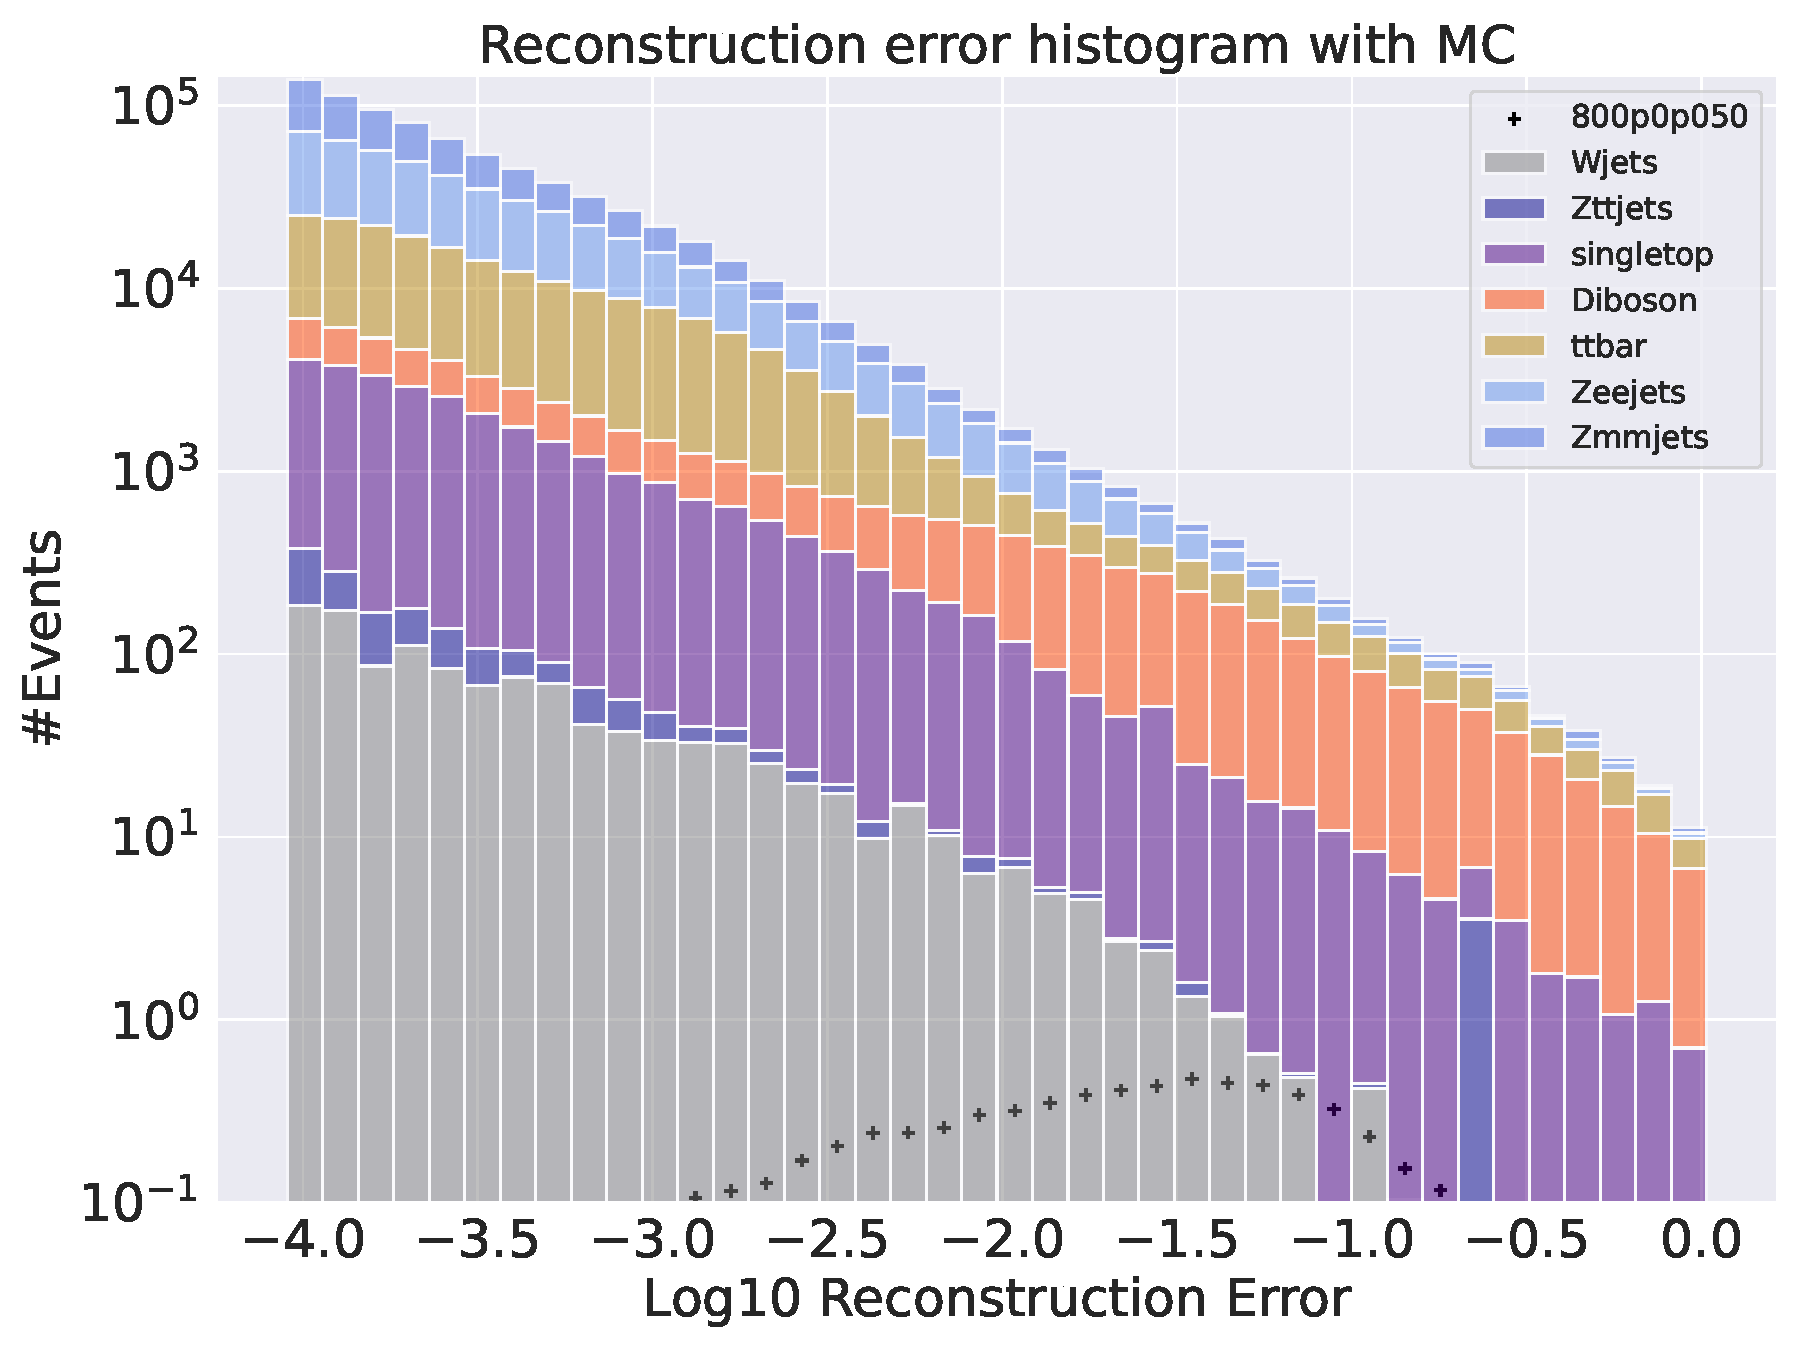
\includegraphics[width=\textwidth]{Figures/AE_testing/small/2lep/b_data_recon_big_rm3_feats_sig_800p0p050_.pdf}
        \caption{ }
        \label{fig:AE_2lep_small_800}
    \end{subfigure}
    \hfill
    \begin{subfigure}{.49\textwidth}
        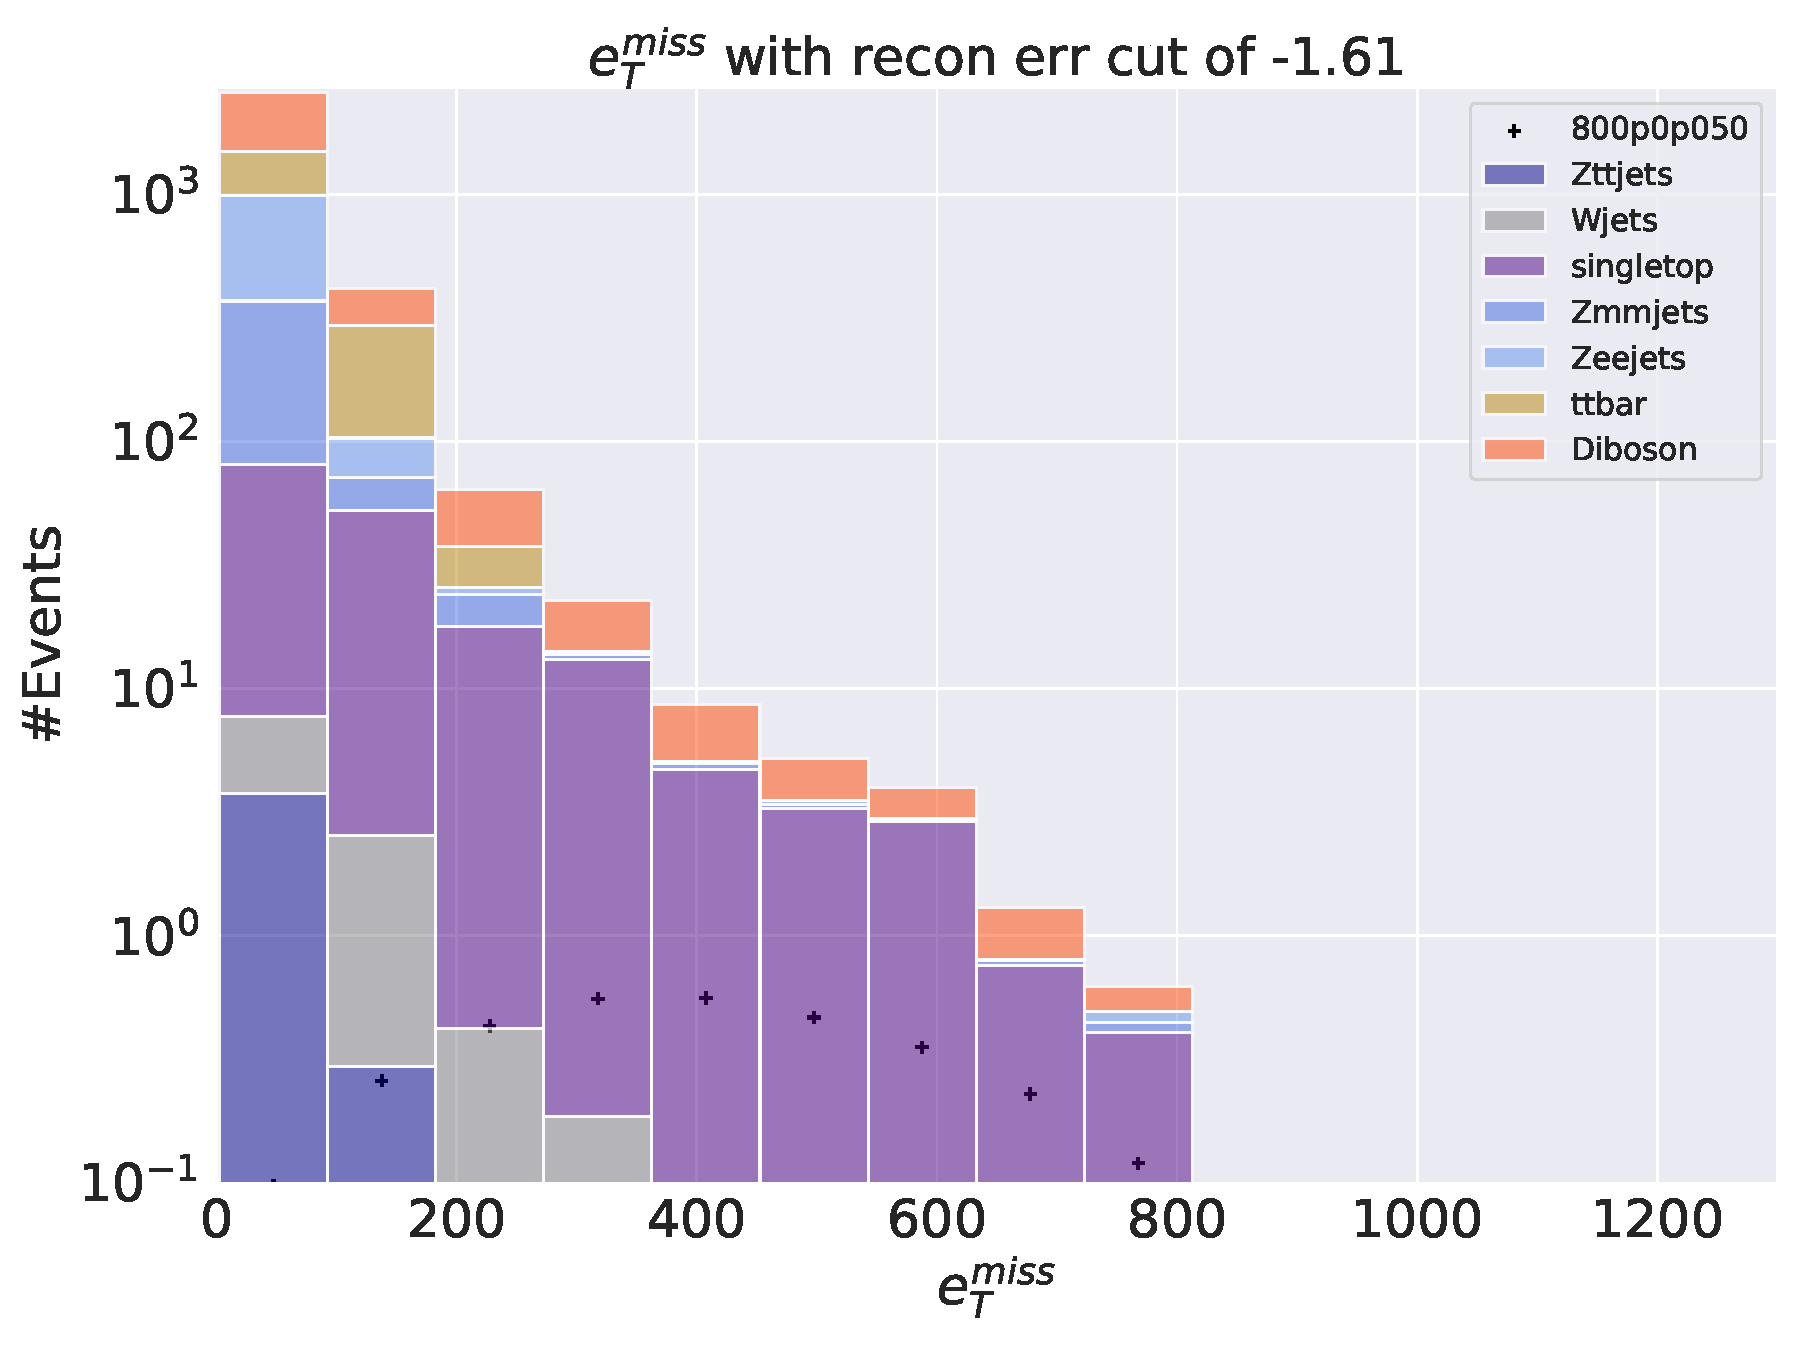
\includegraphics[width=\textwidth]{Figures/AE_testing/small/2lep/b_data_recon_big_rm3_feats_sig_800p0p050_recon_errcut_-1.61.pdf}
        \caption{}
        \label{fig:AE_2lep_small_etmiss_800}
    \end{subfigure}
    \hfill  
    \begin{subfigure}{.49\textwidth}
        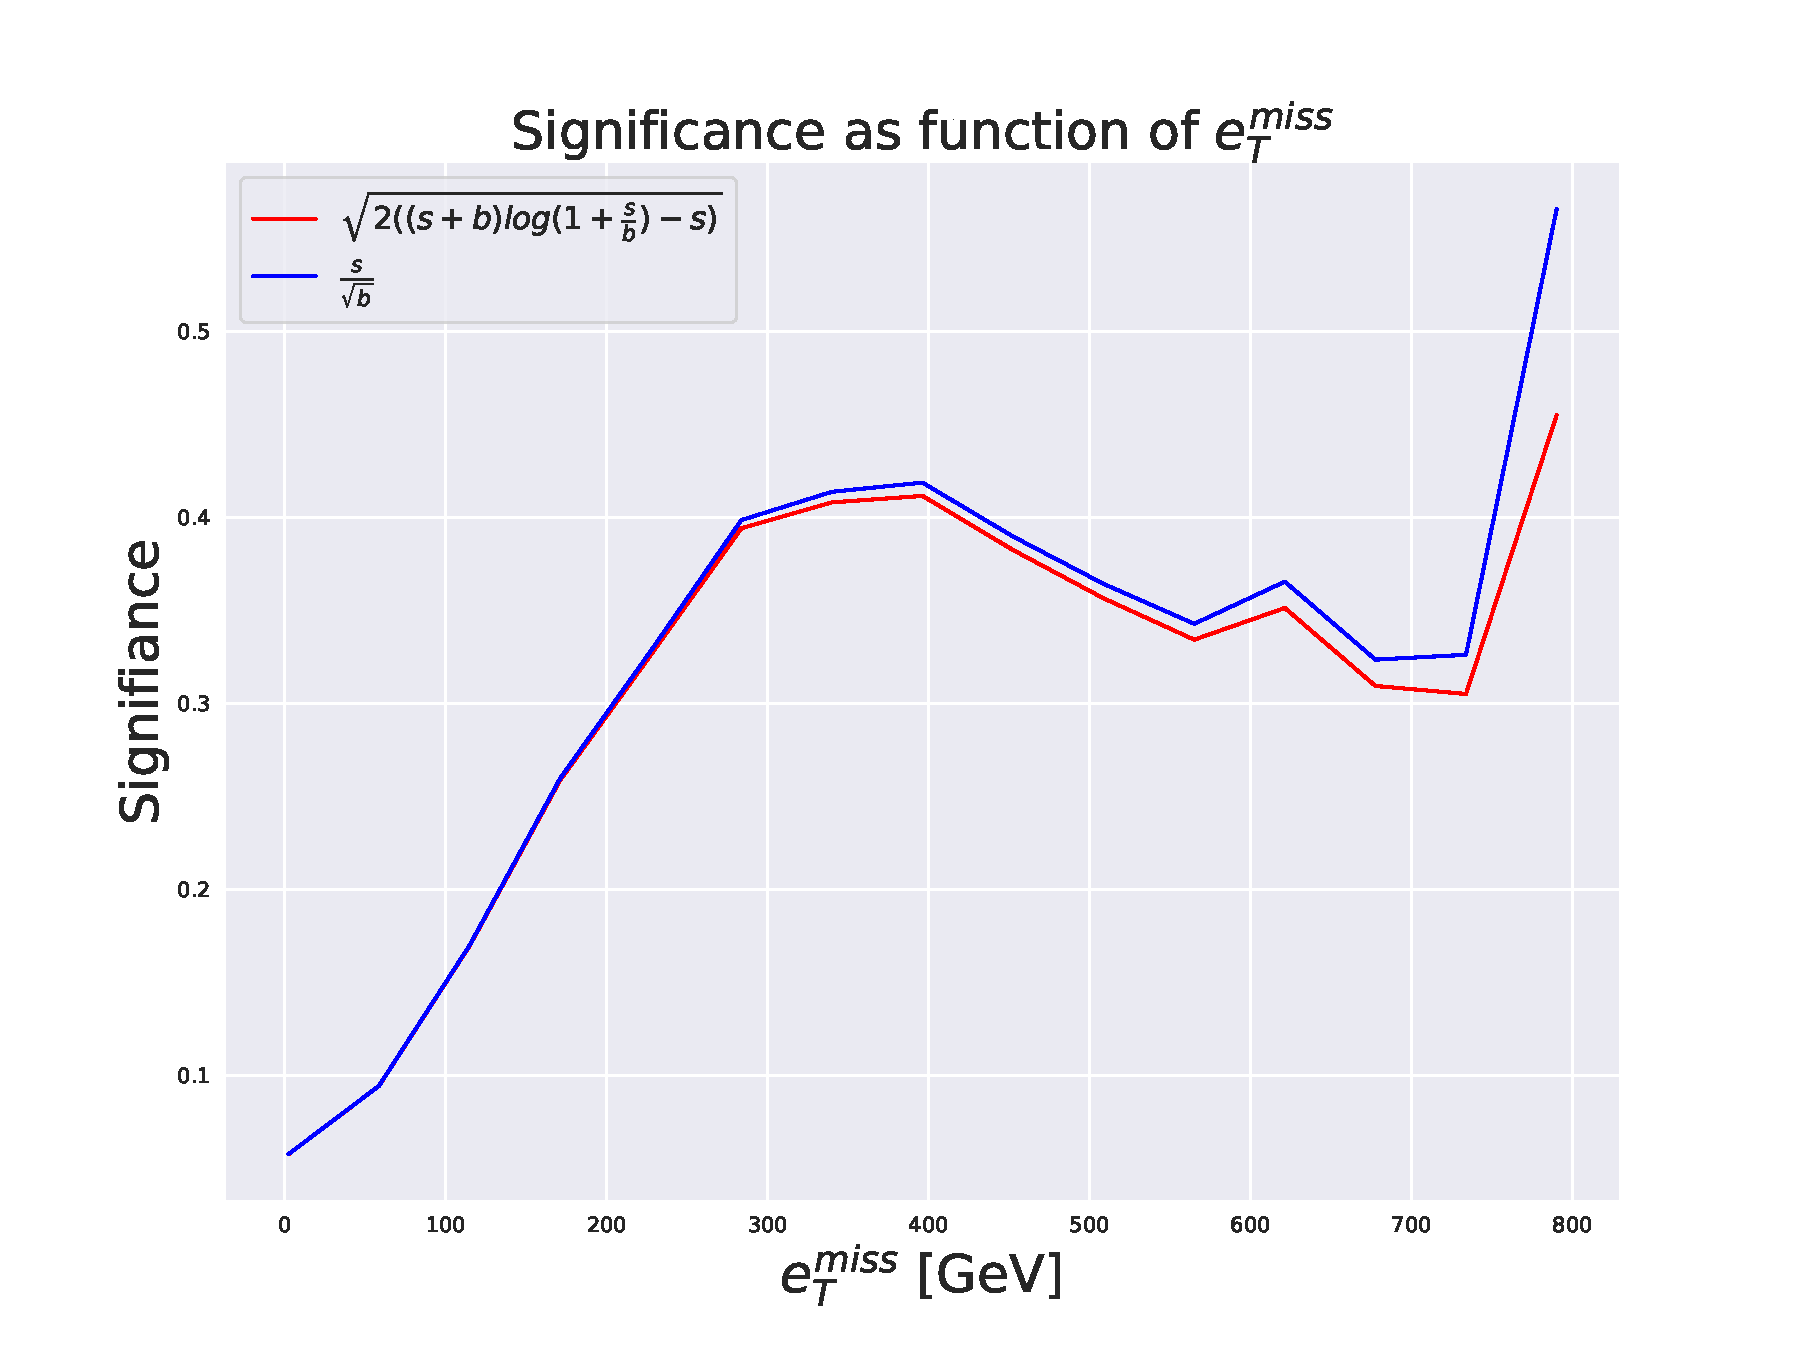
\includegraphics[width=\textwidth]{Figures/AE_testing/small/2lep/significance_etmiss_800p0p050_-1.6117055611472277.pdf}
        \caption{}
        \label{fig:AE_2lep_small_signi_800}
    \end{subfigure}
    \hfill      
    \caption[2lep shallow network | $800p50$ | AE]{Reconstruction error (a), $e_T^{miss}$ signal region (b) and significance as function of 
    $e_T^{miss}$ (c) for the shallow regular autoencoder using SUSY $800p50$. 
    (a) shows the reconstruction error distribution for the SM MC and the SUSY signal. 
    The autoencoder produces a slope-like shape that is highly shifted to the lower end of the reconstruction error range
for the background. The signal is more evenly spread out along the x-axis. The peaks of the two distributions are totally separated
with two orders of magnitude in reconstruction error. (b) shows the $e_T^{miss}$
T distribution for the SM MC and the SUSY signal in the signal region. The signal region is made using a cut around
$10^{-1.61}$. Most of the background is removed, and the peaks of the SM MC and signal distributions are
somewhat separated. (c) shows the significance as function of $e_T^{miss}$. The peak is put 
around a cut of about 400 GeV in the $e_T^{miss}$, with a significance of around $0.42$.}
    \label{fig:AE_2lep_small_rec_sig_signi_800}
\end{figure}


In figures \ref{fig:AE_2lep_big_rec_sig_signi_450}, \ref{fig:AE_2lep_small_rec_sig_signi_450}, 
\ref{fig:AE_2lep_big_rec_sig_signi_800} and \ref{fig:AE_2lep_small_rec_sig_signi_800} we have three 
subplots containing the total reconstruction error distributions, the $e_T^{miss}$ signal region, 
and the significance as function of $e_T^{miss}$ curve respectively. They were created using 
the shallow and deep regular autoencoder with the 2 lepton + $e_T^{miss}$ dataset.
In figures \ref{fig:AE_2lep_big_450}, \ref{fig:AE_2lep_small_450}, \ref{fig:AE_2lep_big_800}, 
\ref{fig:AE_2lep_small_800} there is a continuing trend following the 3 
lepton + $e_T^{miss}$ case shown in figures \ref{fig:AE_3lep_big_450}, \ref{fig:AE_3lep_small_450},
\ref{fig:AE_3lep_big_800}, \ref{fig:AE_3lep_small_800}. This indicates that as we increase the 
statistics, in other words the amount of background events 
used for training, the ability of the autoencoder to learn the internal structure increases. 
As expected, Zmmjets and Zeejets along with ttbar are the channels with the highest statistics 
in the 2 lepton + $e_T^{miss}$ dataset, thus it should be easier to learn to better reconstruct 
those events. However, note the amount of diboson in the higher end of the reconstruction error 
histograms, as well as in the $e_T^{miss}$ post reconstruction error cut distributions.  \par
In figures \ref{fig:AE_2lep_big_etmiss_450}, \ref{fig:AE_2lep_small_etmiss_450}, \ref{fig:AE_2lep_big_etmiss_800} and  
\ref{fig:AE_2lep_small_etmiss_800} we have the $e_T^{miss}$ distributions for 
the least strict cuts for the regular autoencoder models. One indication that the search strategy 
used in this thesis could work is if the models can improve the significance from just looking at 
the $e_T^{miss}$ distributions of the background and the signal in mind. Thus, we want to compare the pre 
reconstruction error significance with the signal region based on the autoencoder output. The significance 
in the pre reconstruction error case were for the SUSY $450p300$ signal 0.017 using both 
the small and large statistics formula, and 0.0014 for the SUSY $800p50$ signal. Note here that for 
$e_T^{miss}$, no physics informed cuts have been used, but there are certain cuts that can increase 
the significance, so the significance in should be considered to possibly be somewhat higher. \par
In figures \ref{fig:AE_2lep_big_signi_450}, \ref{fig:AE_2lep_small_signi_450}, \ref{fig:AE_2lep_big_signi_800} 
and  \ref{fig:AE_2lep_small_signi_800} we have the significance as function of $e_T^{miss}$. 
This plot shows an increased significance when applying an additional cut in the $e_T^{miss}$ distribution.
The highest significance was found with the shallow autoencoder with the SUSY $450p300$ signal model. 
It should be noted that the significance 
for the $800p50$ signal model is a lot smaller than for the $450p300$ signal model, even though the separation 
shown in figures \ref{fig:AE_2lep_big_450}, \ref{fig:AE_2lep_small_450}, \ref{fig:AE_2lep_big_800}, 
\ref{fig:AE_2lep_small_800} would suggest otherwise. The reason for the low significance is that the cross-section is 
much lower for the $800p50$ signal. The peak in both signal models are fairly 
separated from the peak of the SM MC, the SUSY $800p50$ signal model is shifted a bit more to the right end. 

\par

\subsubsection*{Variational autoencoder performance}

\begin{figure}[h!]
    \centering
    \begin{subfigure}{.49\textwidth}
        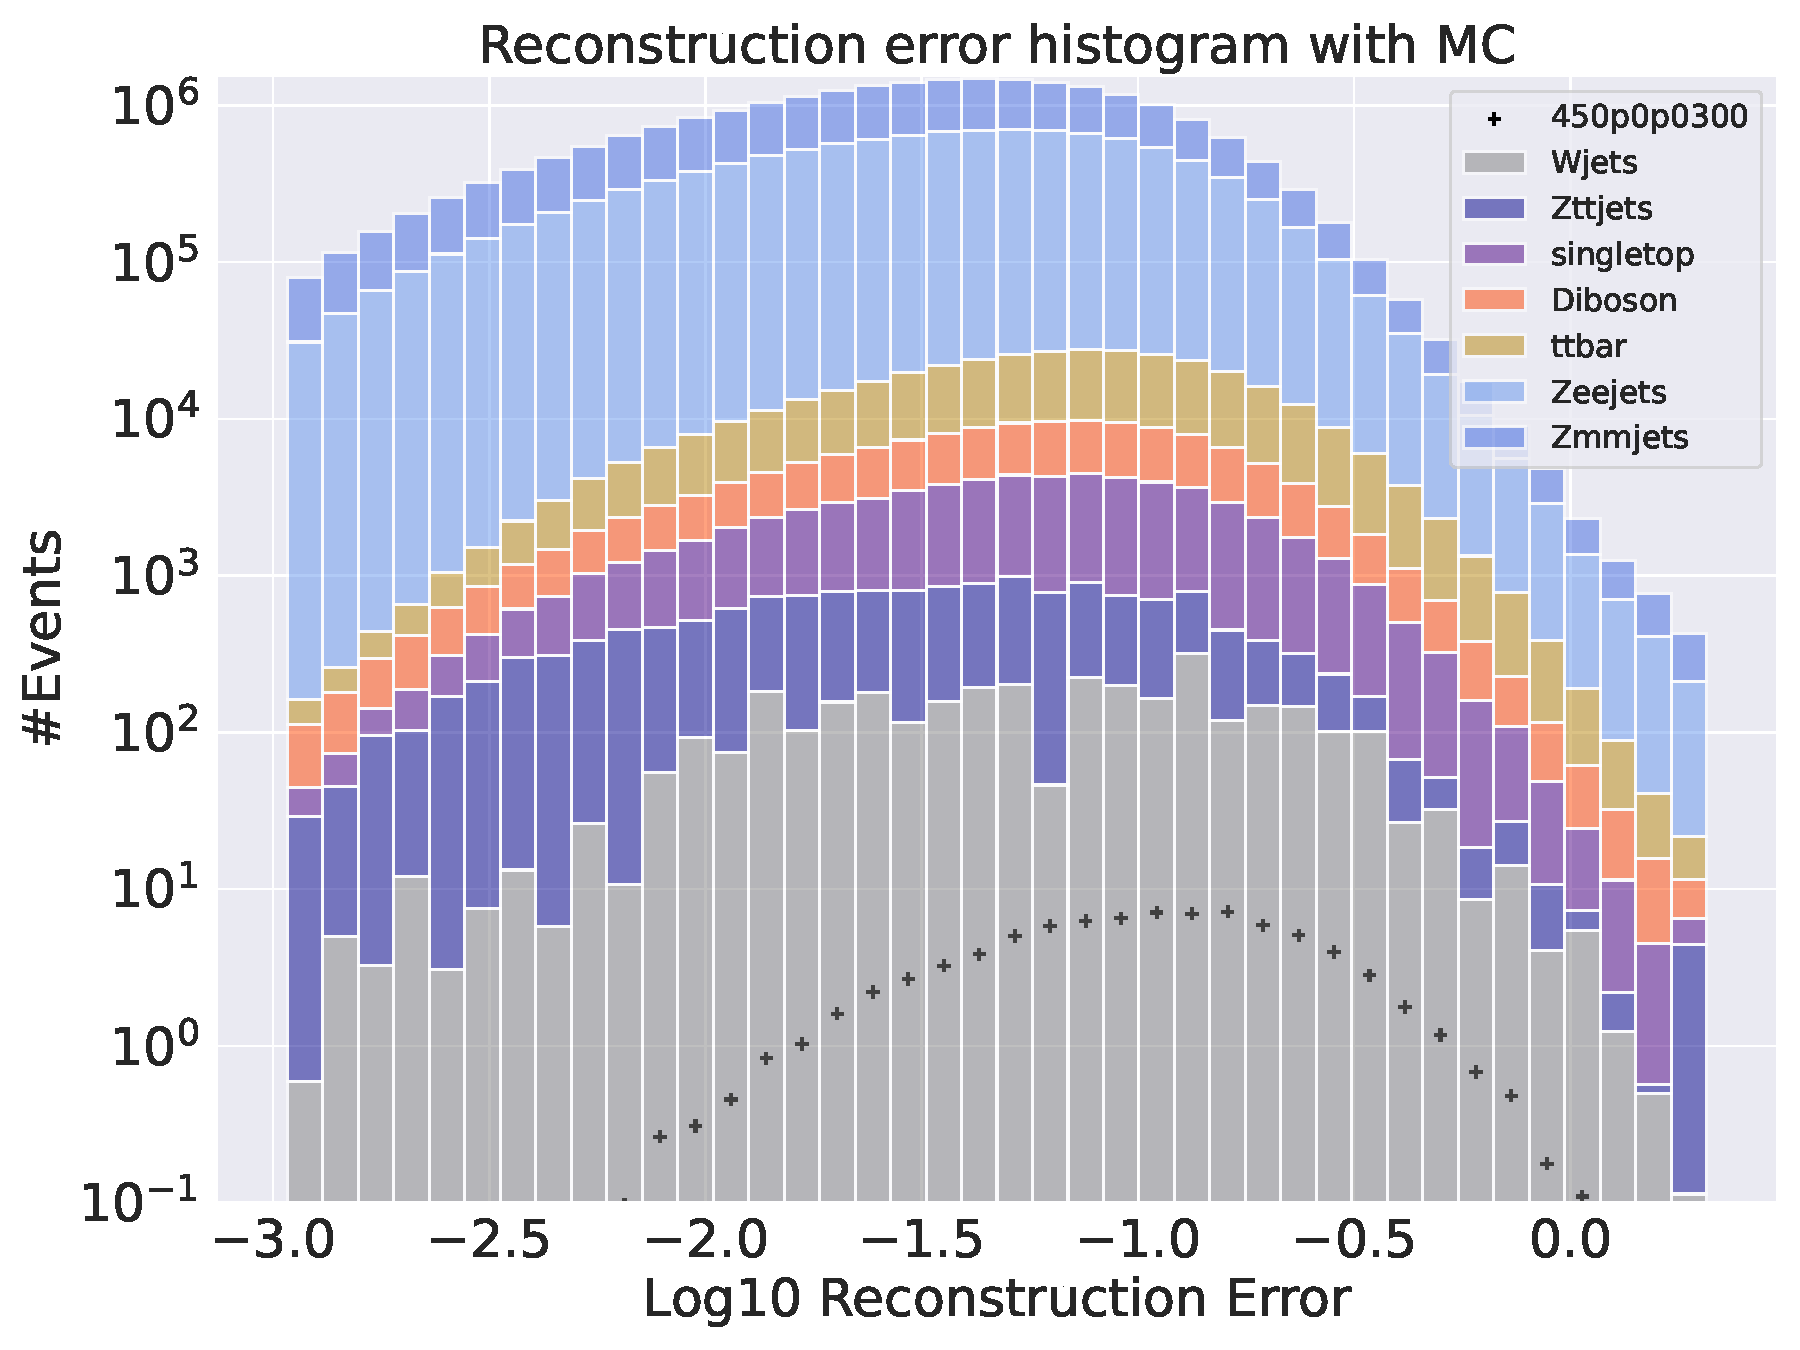
\includegraphics[width=\textwidth]{Figures/VAE_testing/small/2lep/b_data_recon_big_rm3_feats_sig_450p0p0300_.pdf}
        \caption{ }
        \label{fig:VAE_2lep_big_450}
    \end{subfigure}
    \hfill
    \begin{subfigure}{.49\textwidth}
        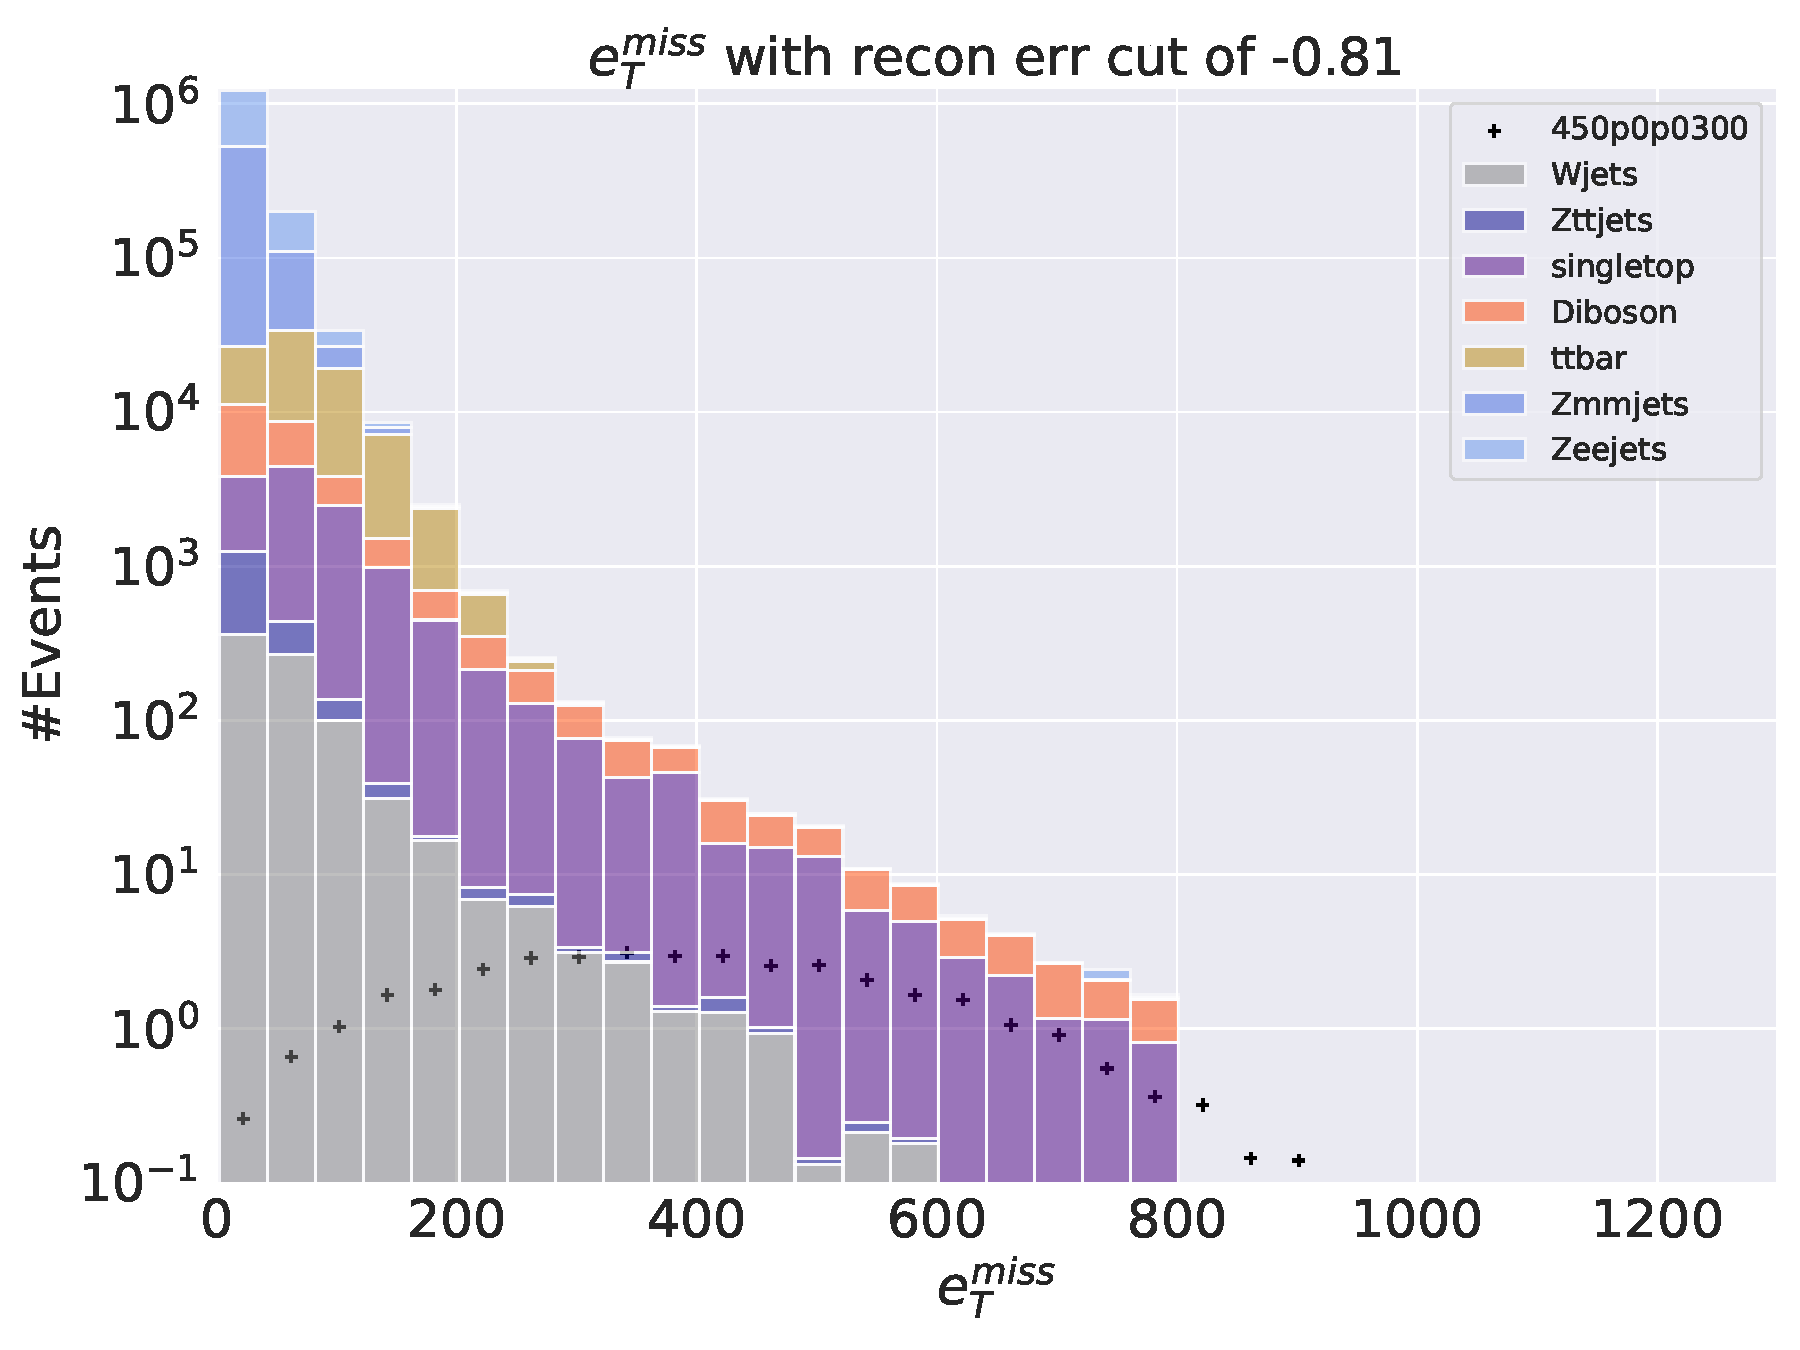
\includegraphics[width=\textwidth]{Figures/VAE_testing/big/2lep/b_data_recon_big_rm3_feats_sig_450p0p0300_recon_errcut_-0.81.pdf}
        \caption{}
        \label{fig:VAE_2lep_big_etmiss_450}
    \end{subfigure}
    \hfill 
    \begin{subfigure}{.49\textwidth}
        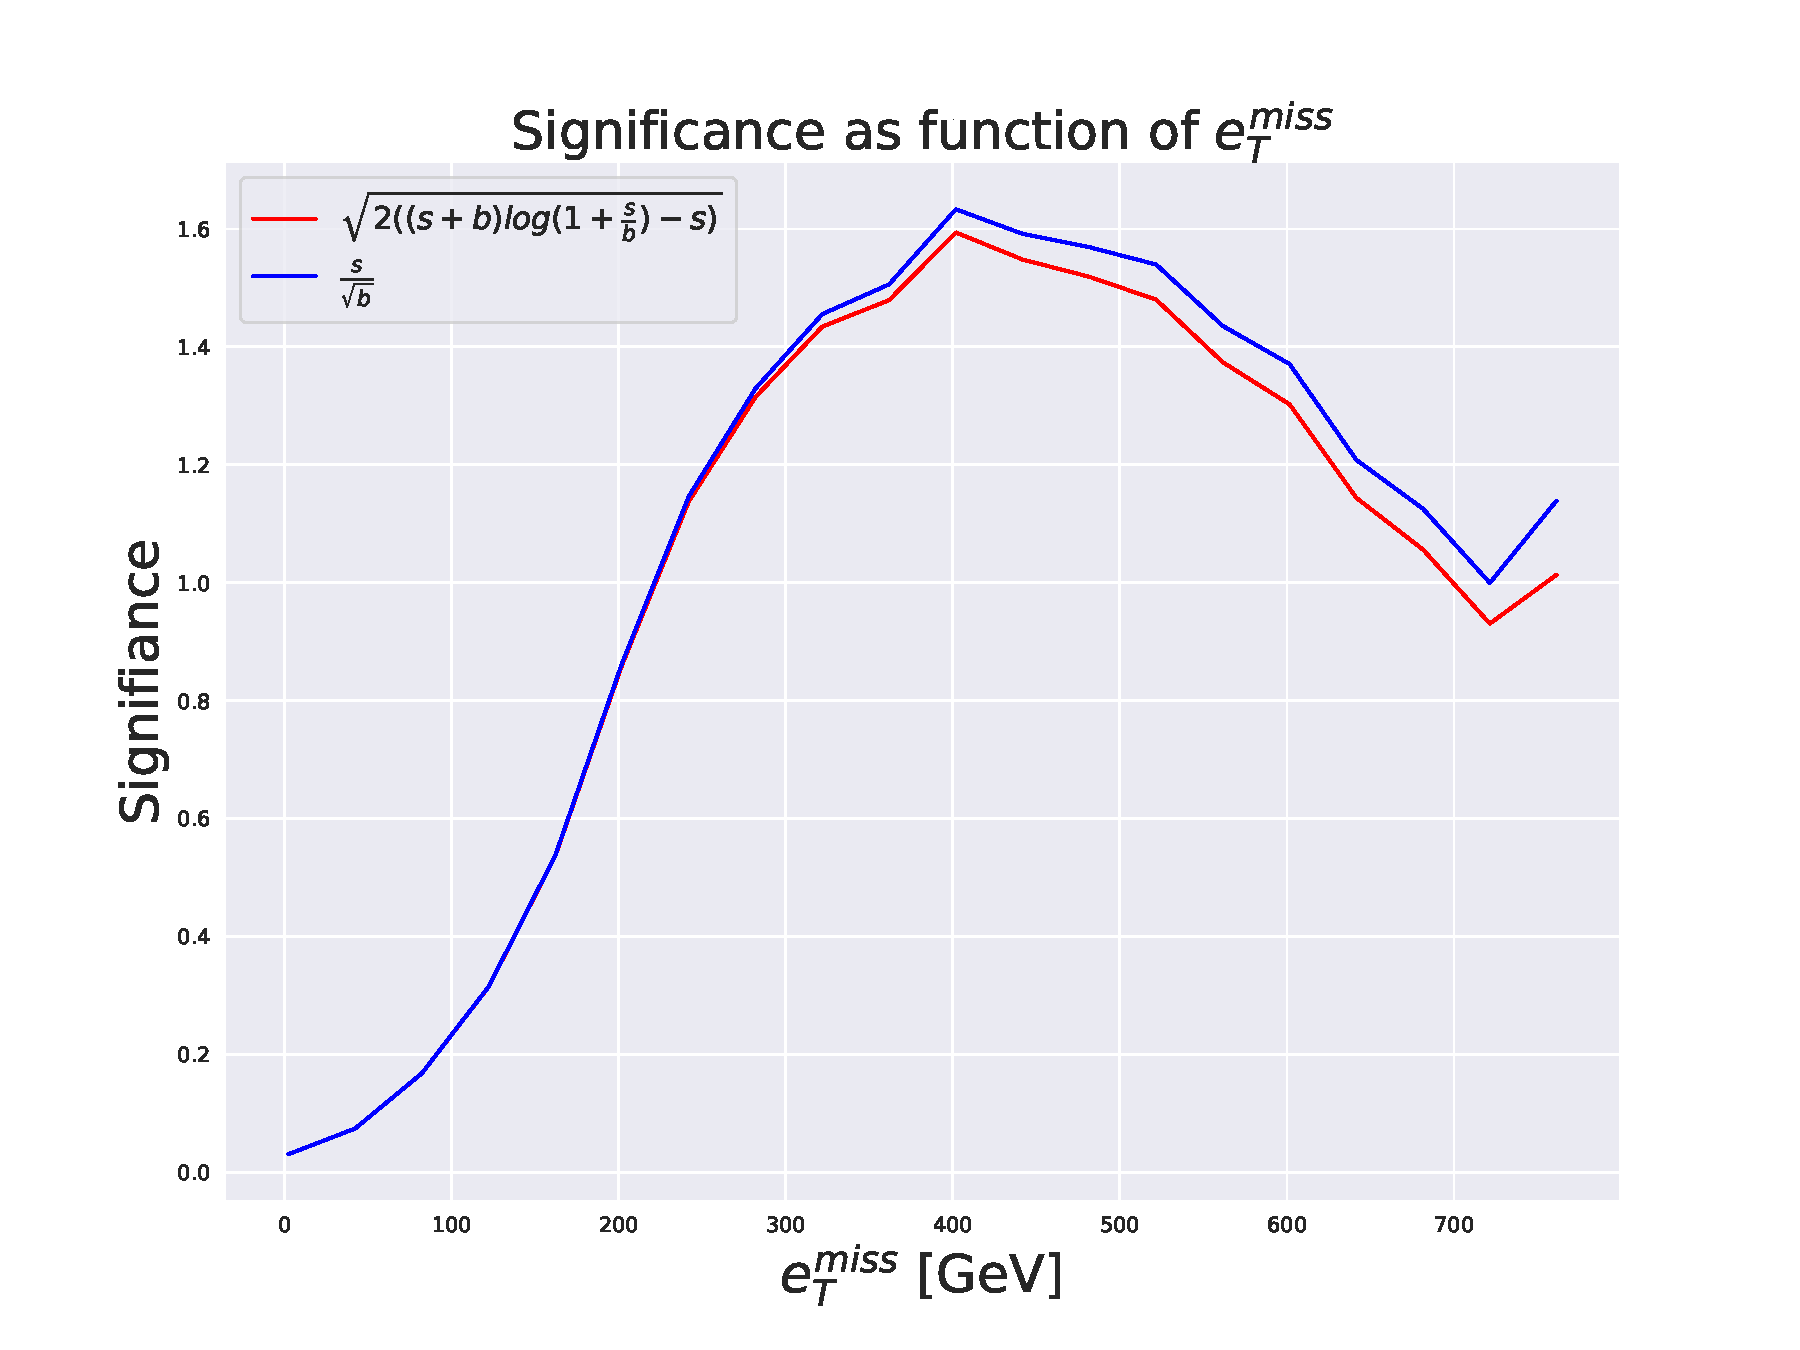
\includegraphics[width=\textwidth]{Figures/VAE_testing/big/2lep/significance_etmiss_450p0p0300_-0.8121874101107931.pdf}
        \caption{}
        \label{fig:VAE_2lep_big_signi_450}
    \end{subfigure}
    \hfill      
    \caption[2lep deep network | $450p300$ | VAE]{Reconstruction error (a), $e_T^{miss}$ signal region (b) and significance as function of 
    $e_T^{miss}$ (c) for the deep regular autoencoder using SUSY $450p300$. 
    (a) shows that the peak of the distribution is somewhat centered in the middle 
    of the reconstruction error range forming a hill-like shape. The peaks of the background and signal 
    distributions are not well separated, with almost identical reconstruction error pattern. (b) 
    shows a signal region with large background distribution. The signal region is made using a cut around
    $10^{-0.81}$. The peaks in the signal region are also somewhat 
    separated, but the overall distributions are overlapping still. 
    (c) shows the significance as function of $e_T^{miss}$. 
    The peak significance is around 1.61 at around 400 GeV.}
    \label{fig:VAE_2lep_big_rec_sig_signi_450}
\end{figure}

\begin{figure}[h!]
    \centering
    \begin{subfigure}{.49\textwidth}
        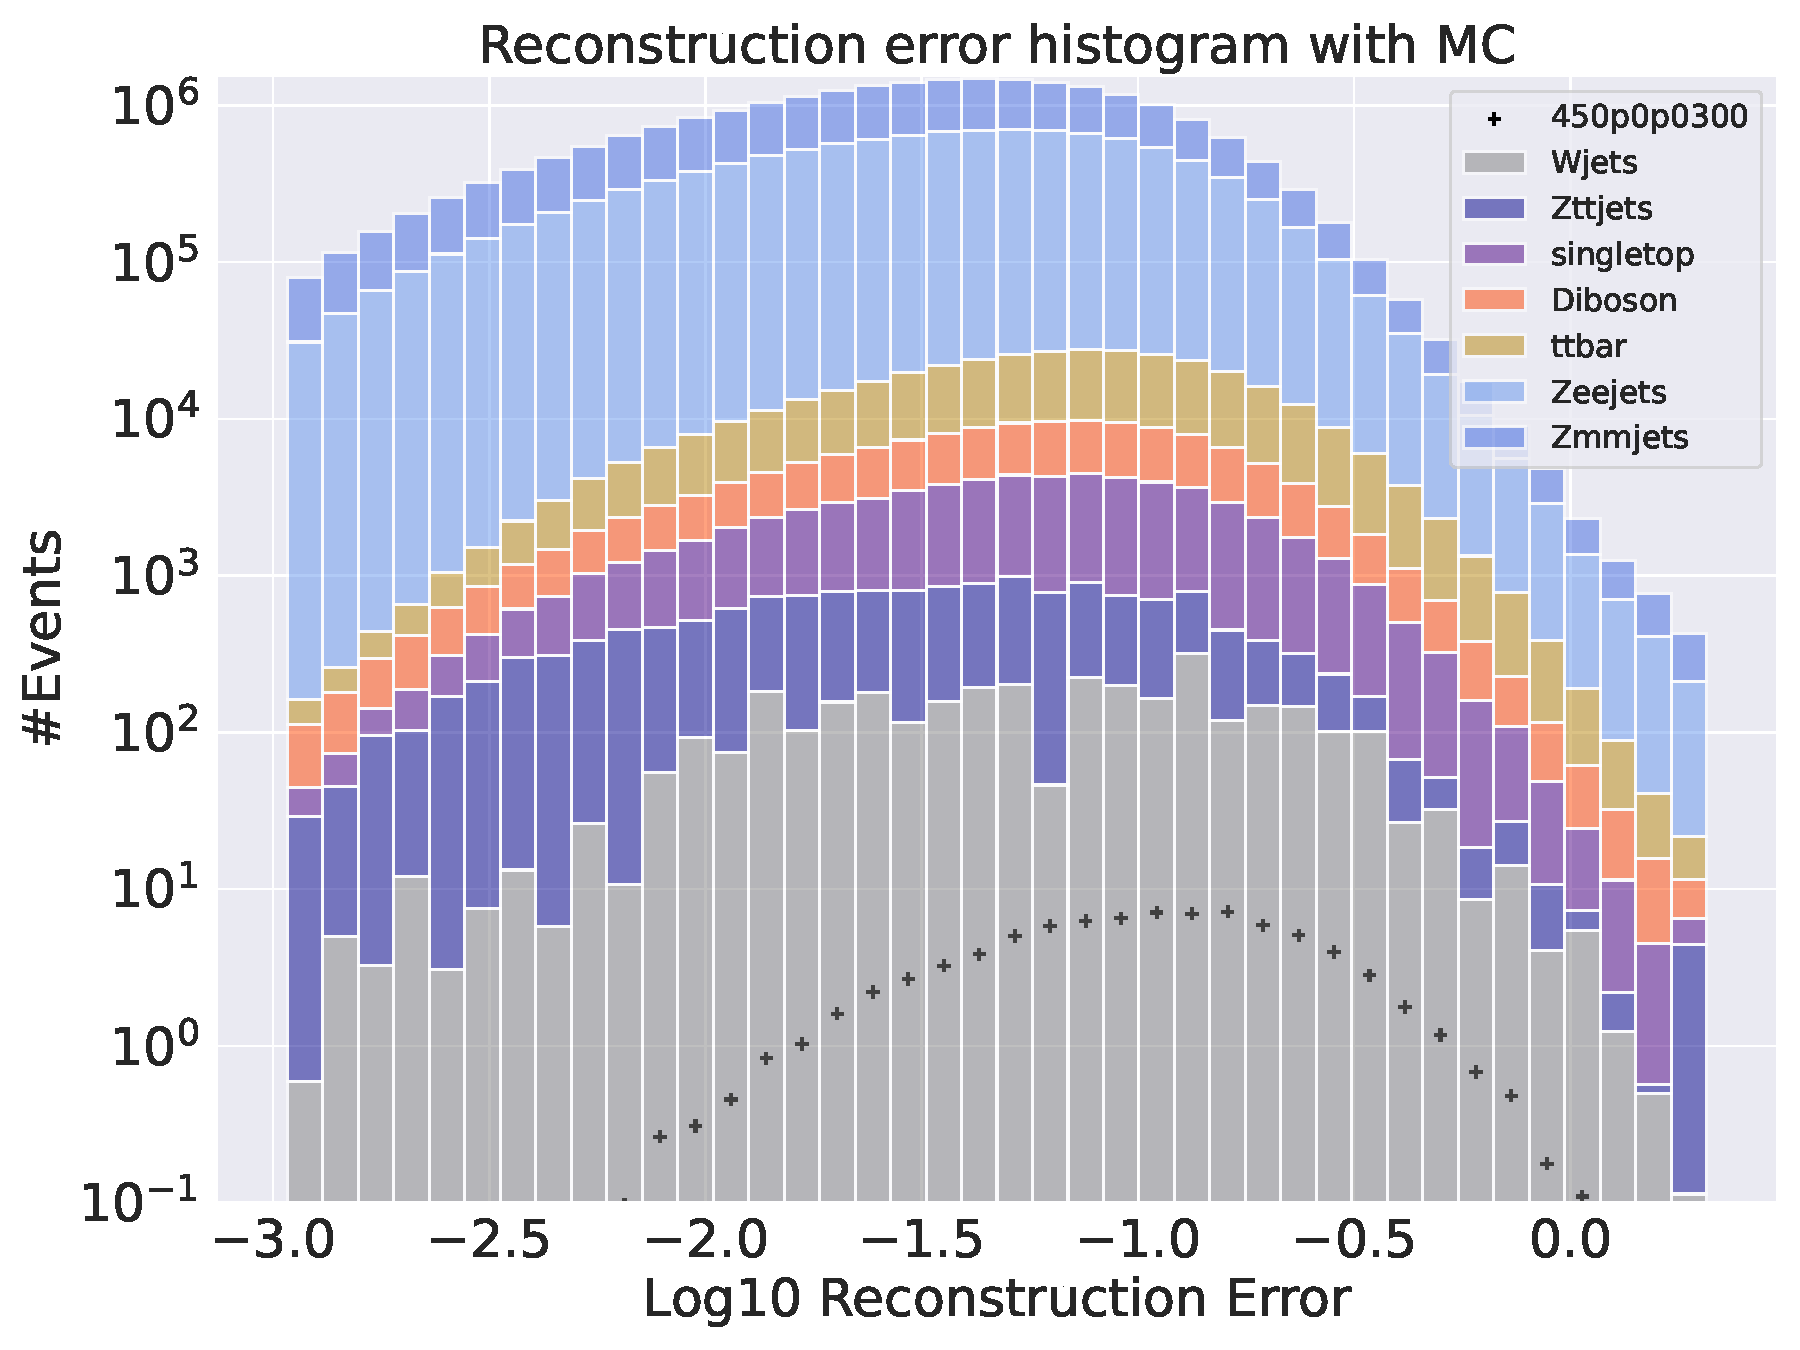
\includegraphics[width=\textwidth]{Figures/VAE_testing/small/2lep/b_data_recon_big_rm3_feats_sig_450p0p0300_.pdf}
        \caption{ }
        \label{fig:VAE_2lep_small_450}
    \end{subfigure}
    \hfill
    \begin{subfigure}{.49\textwidth}
        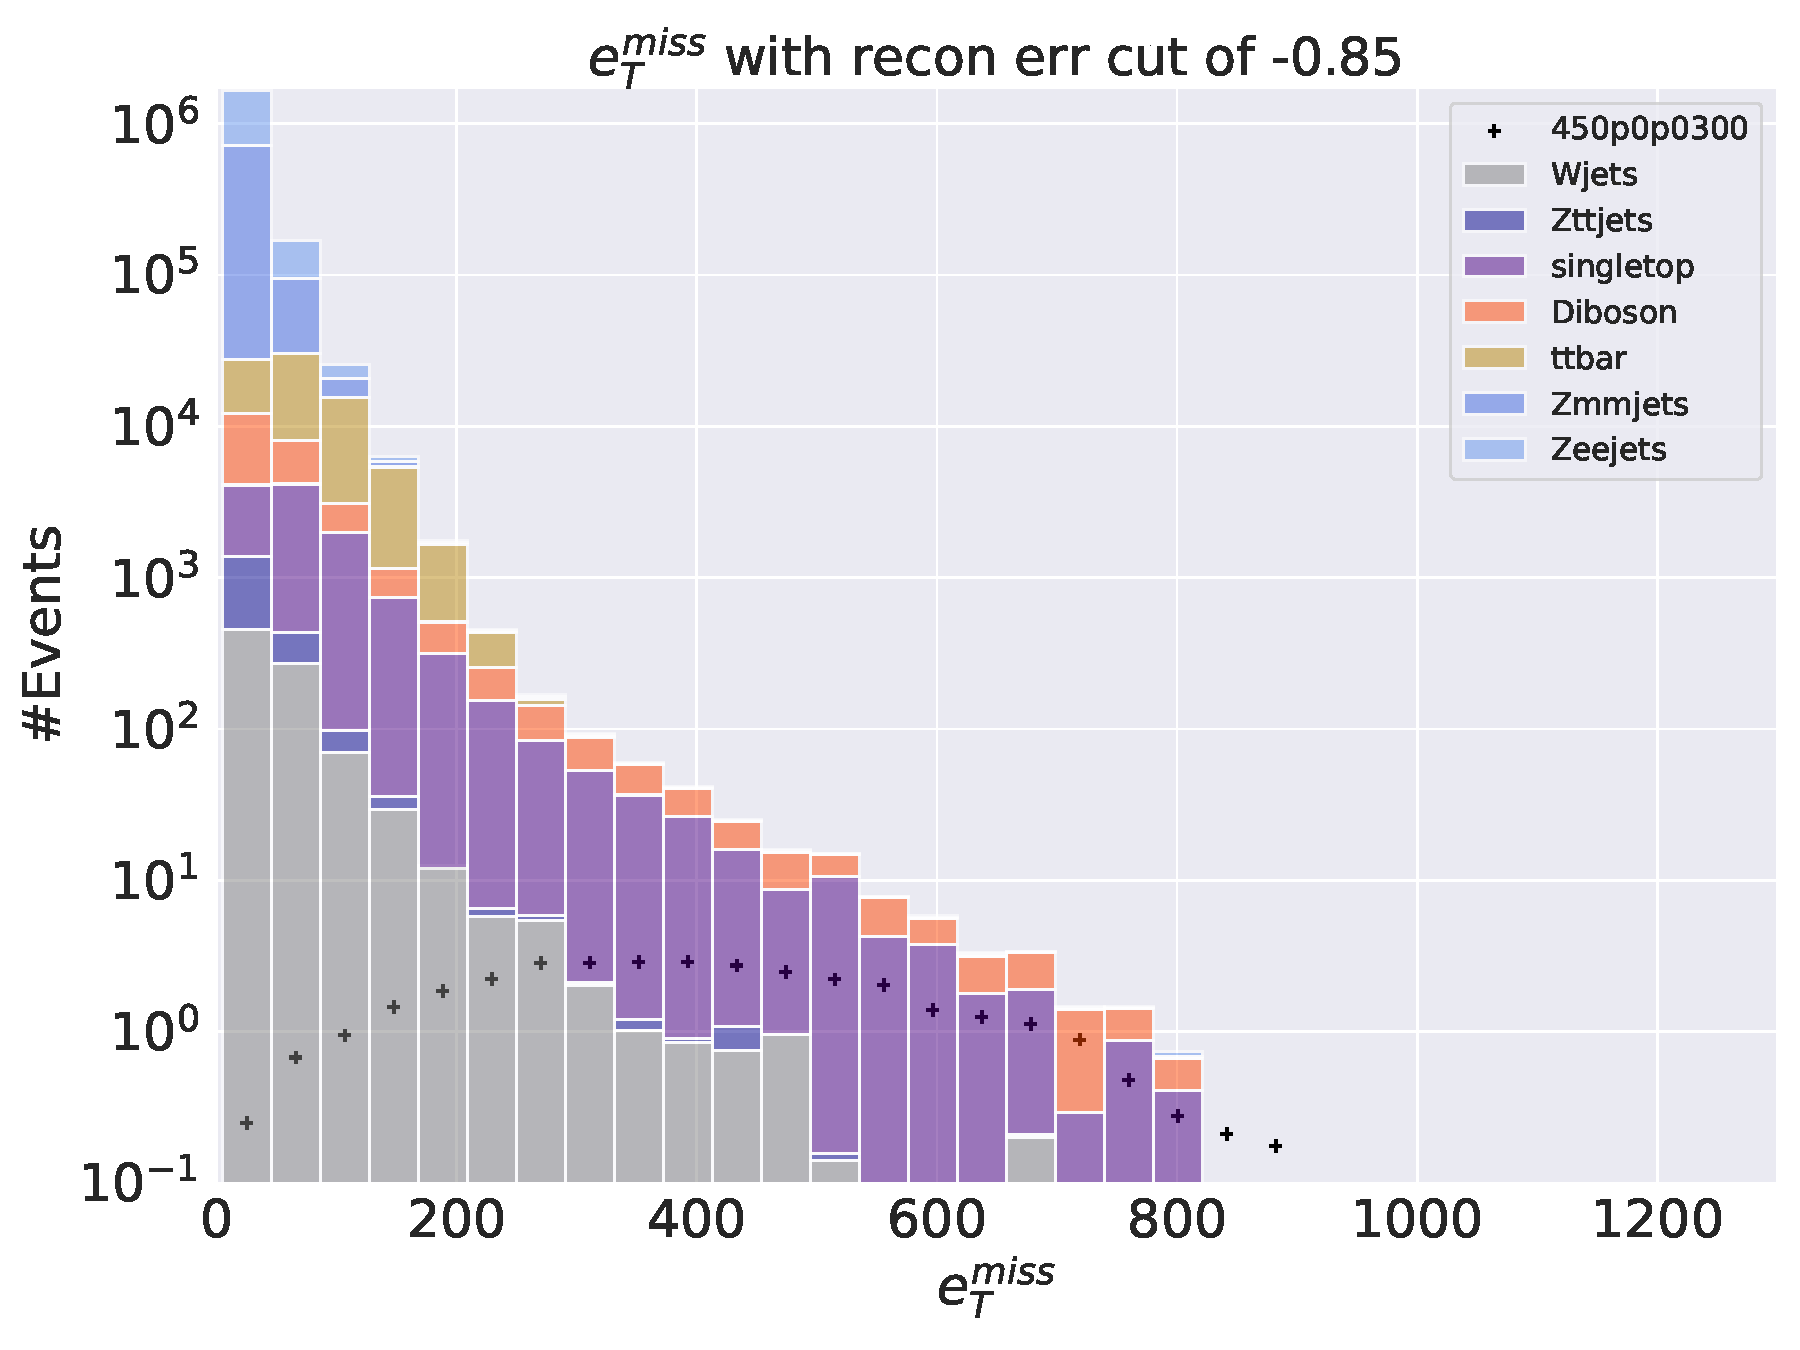
\includegraphics[width=\textwidth]{Figures/VAE_testing/small/2lep/b_data_recon_big_rm3_feats_sig_450p0p0300_recon_errcut_-0.85.pdf}
        \caption{}
        \label{fig:VAE_2lep_small_etmiss_450}
    \end{subfigure}
    \hfill  
    \begin{subfigure}{.49\textwidth}
        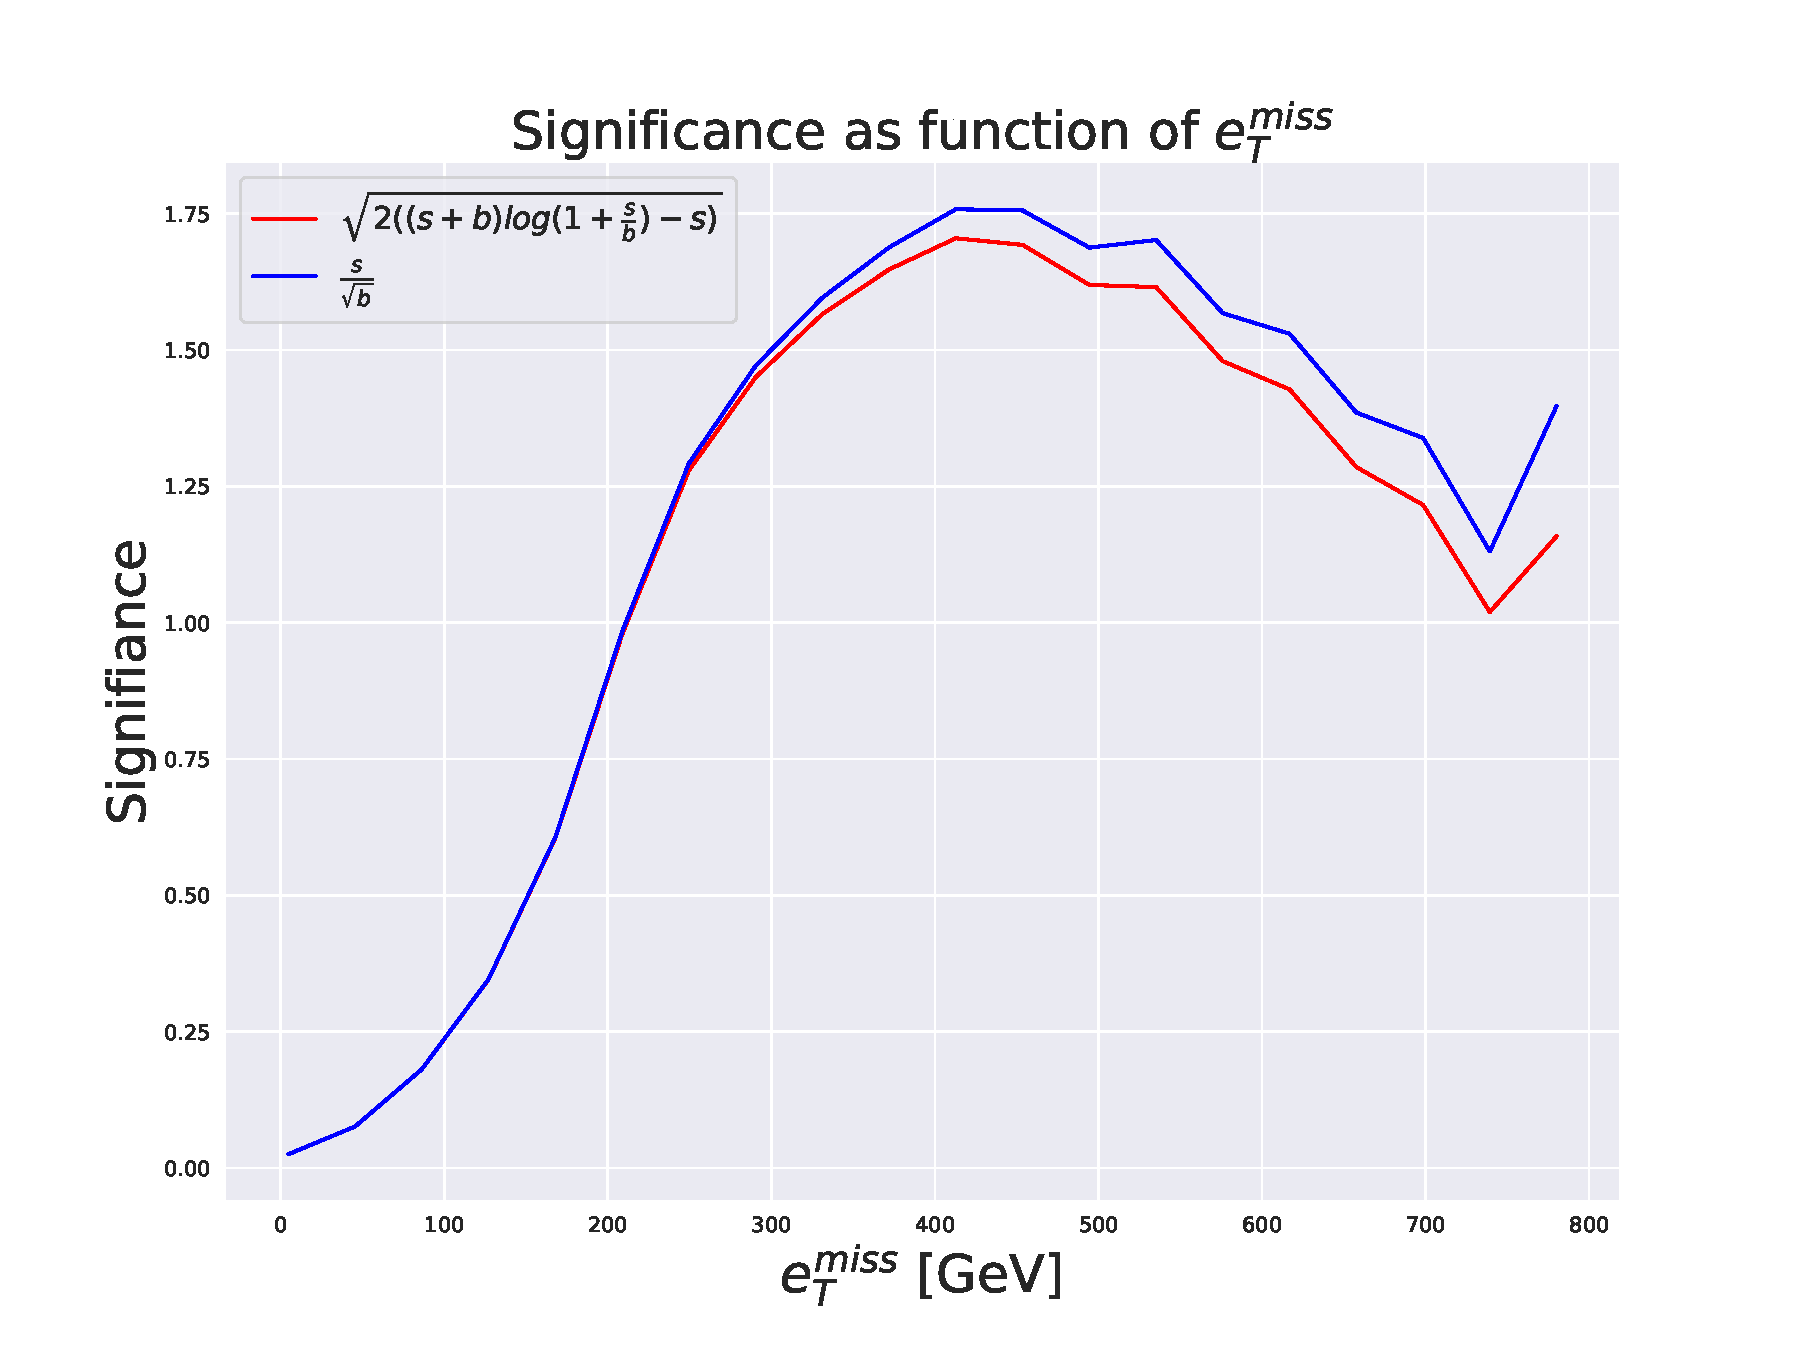
\includegraphics[width=\textwidth]{Figures/VAE_testing/small/2lep/significance_etmiss_450p0p0300_-0.8484803499636524.pdf}
        \caption{}
        \label{fig:VAE_2lep_small_signi_450}
    \end{subfigure}
    \hfill      
    \caption[2lep shallow network | $450p300$ | VAE]{Reconstruction error (a), $e_T^{miss}$ signal region (b) and significance as function of 
    $e_T^{miss}$ (c) for the shallow regular autoencoder using SUSY $450p300$.
    (a) shows that the peak of the distribution is somewhat centered in the middle 
    of the reconstruction error range forming a hill-like shape. The peaks of the background and signal 
    distributions are not well separated, with almost identical reconstruction error pattern. (b) 
    shows a signal region with large background distribution. The signal region is made using a cut around
    $10^{-0.85}$. The peaks in the signal region are also somewhat 
    separated, but the overall distributions are overlapping still. 
    (c) shows the significance as function of $e_T^{miss}$. 
The peak significance is around 1.75 at around 420-450 GeV.}
    \label{fig:VAE_2lep_small_rec_sig_signi_450}
\end{figure}


\begin{figure}[h!]
    \centering
    \begin{subfigure}{.49\textwidth}
        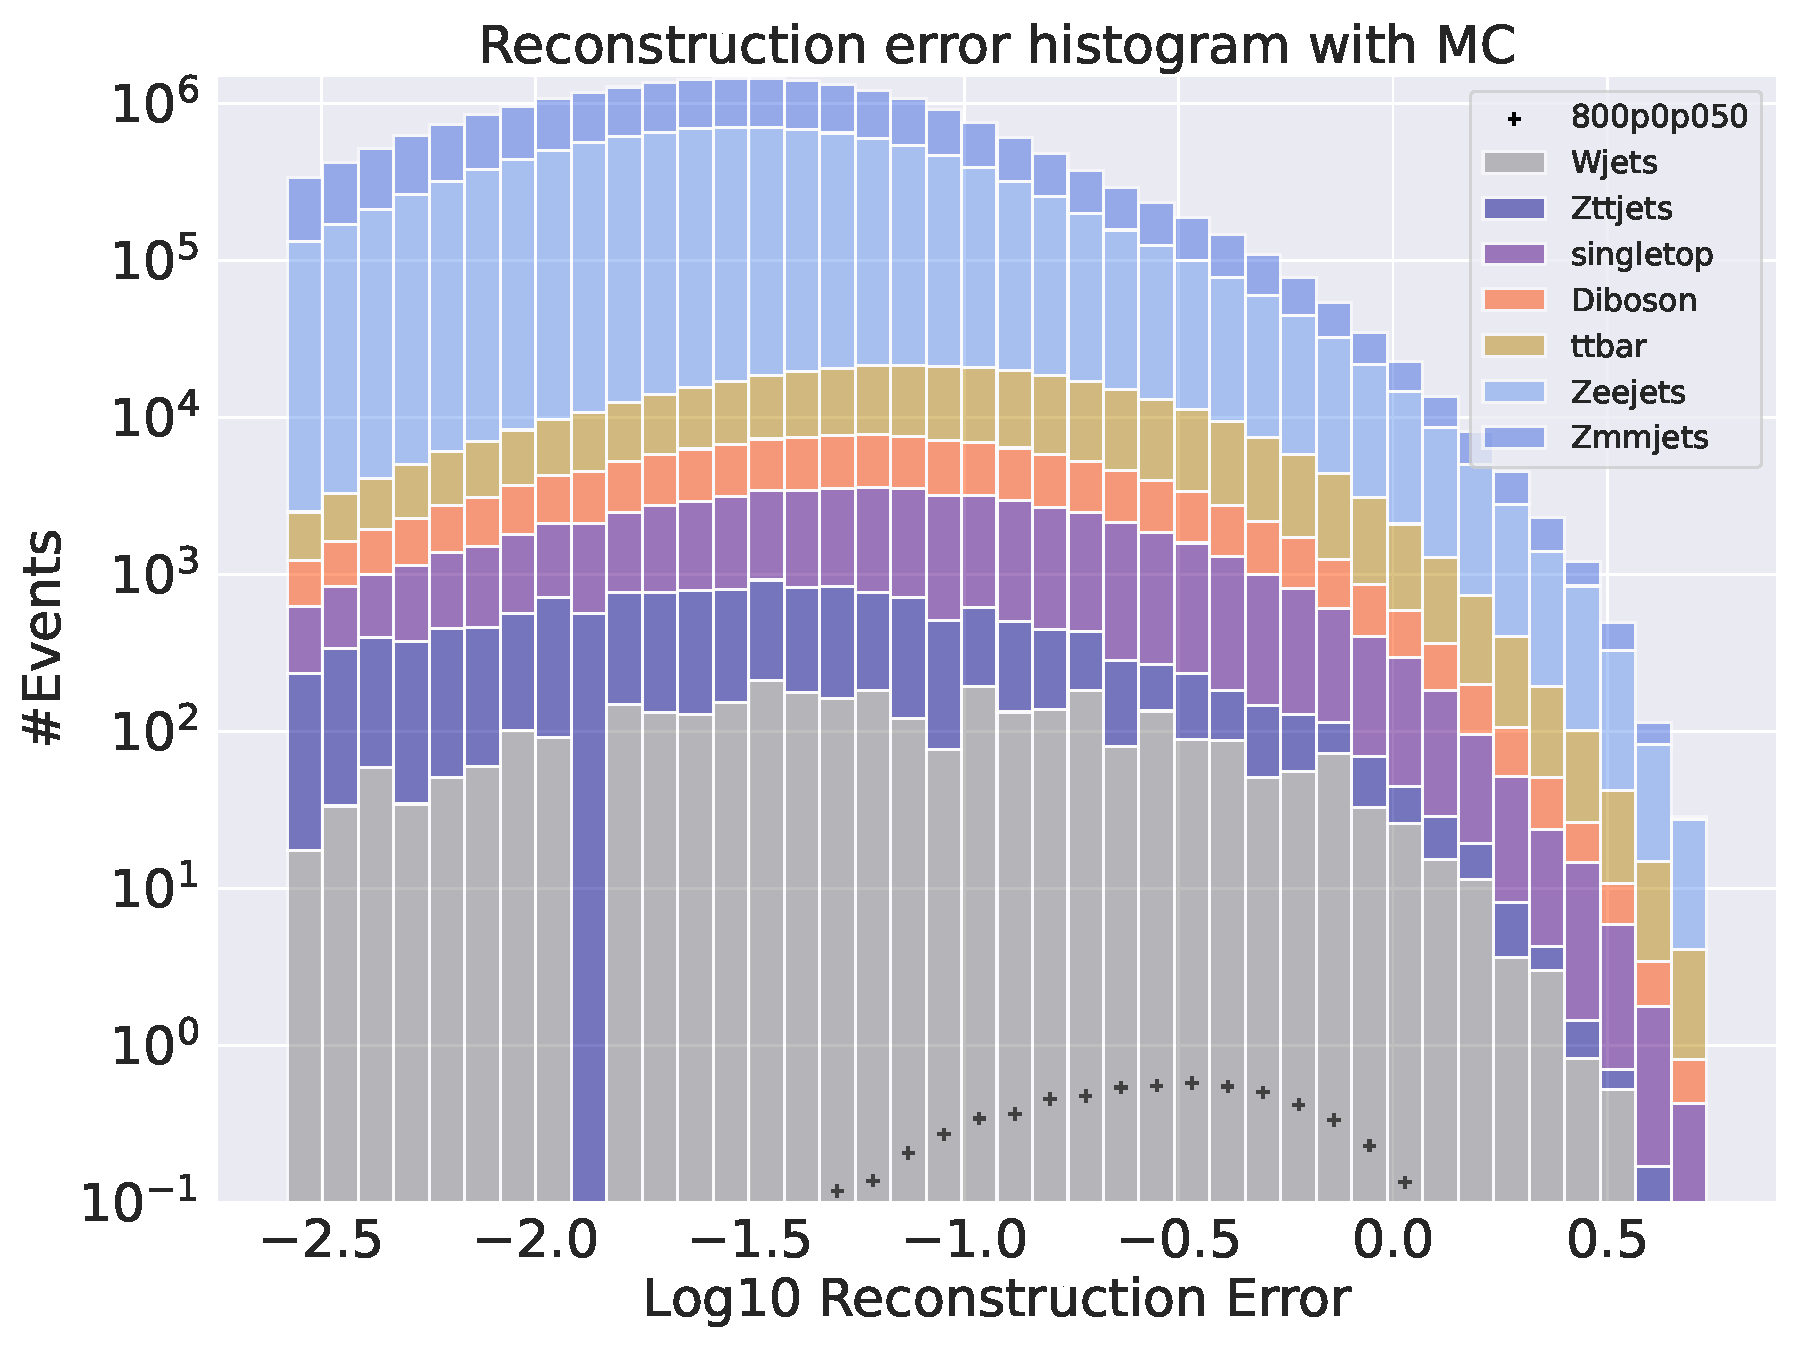
\includegraphics[width=\textwidth]{Figures/VAE_testing/big/2lep/b_data_recon_big_rm3_feats_sig_800p0p050_.pdf}
        \caption{ }
        \label{fig:VAE_2lep_big_800}
    \end{subfigure}
    \hfill
    \begin{subfigure}{.49\textwidth}
        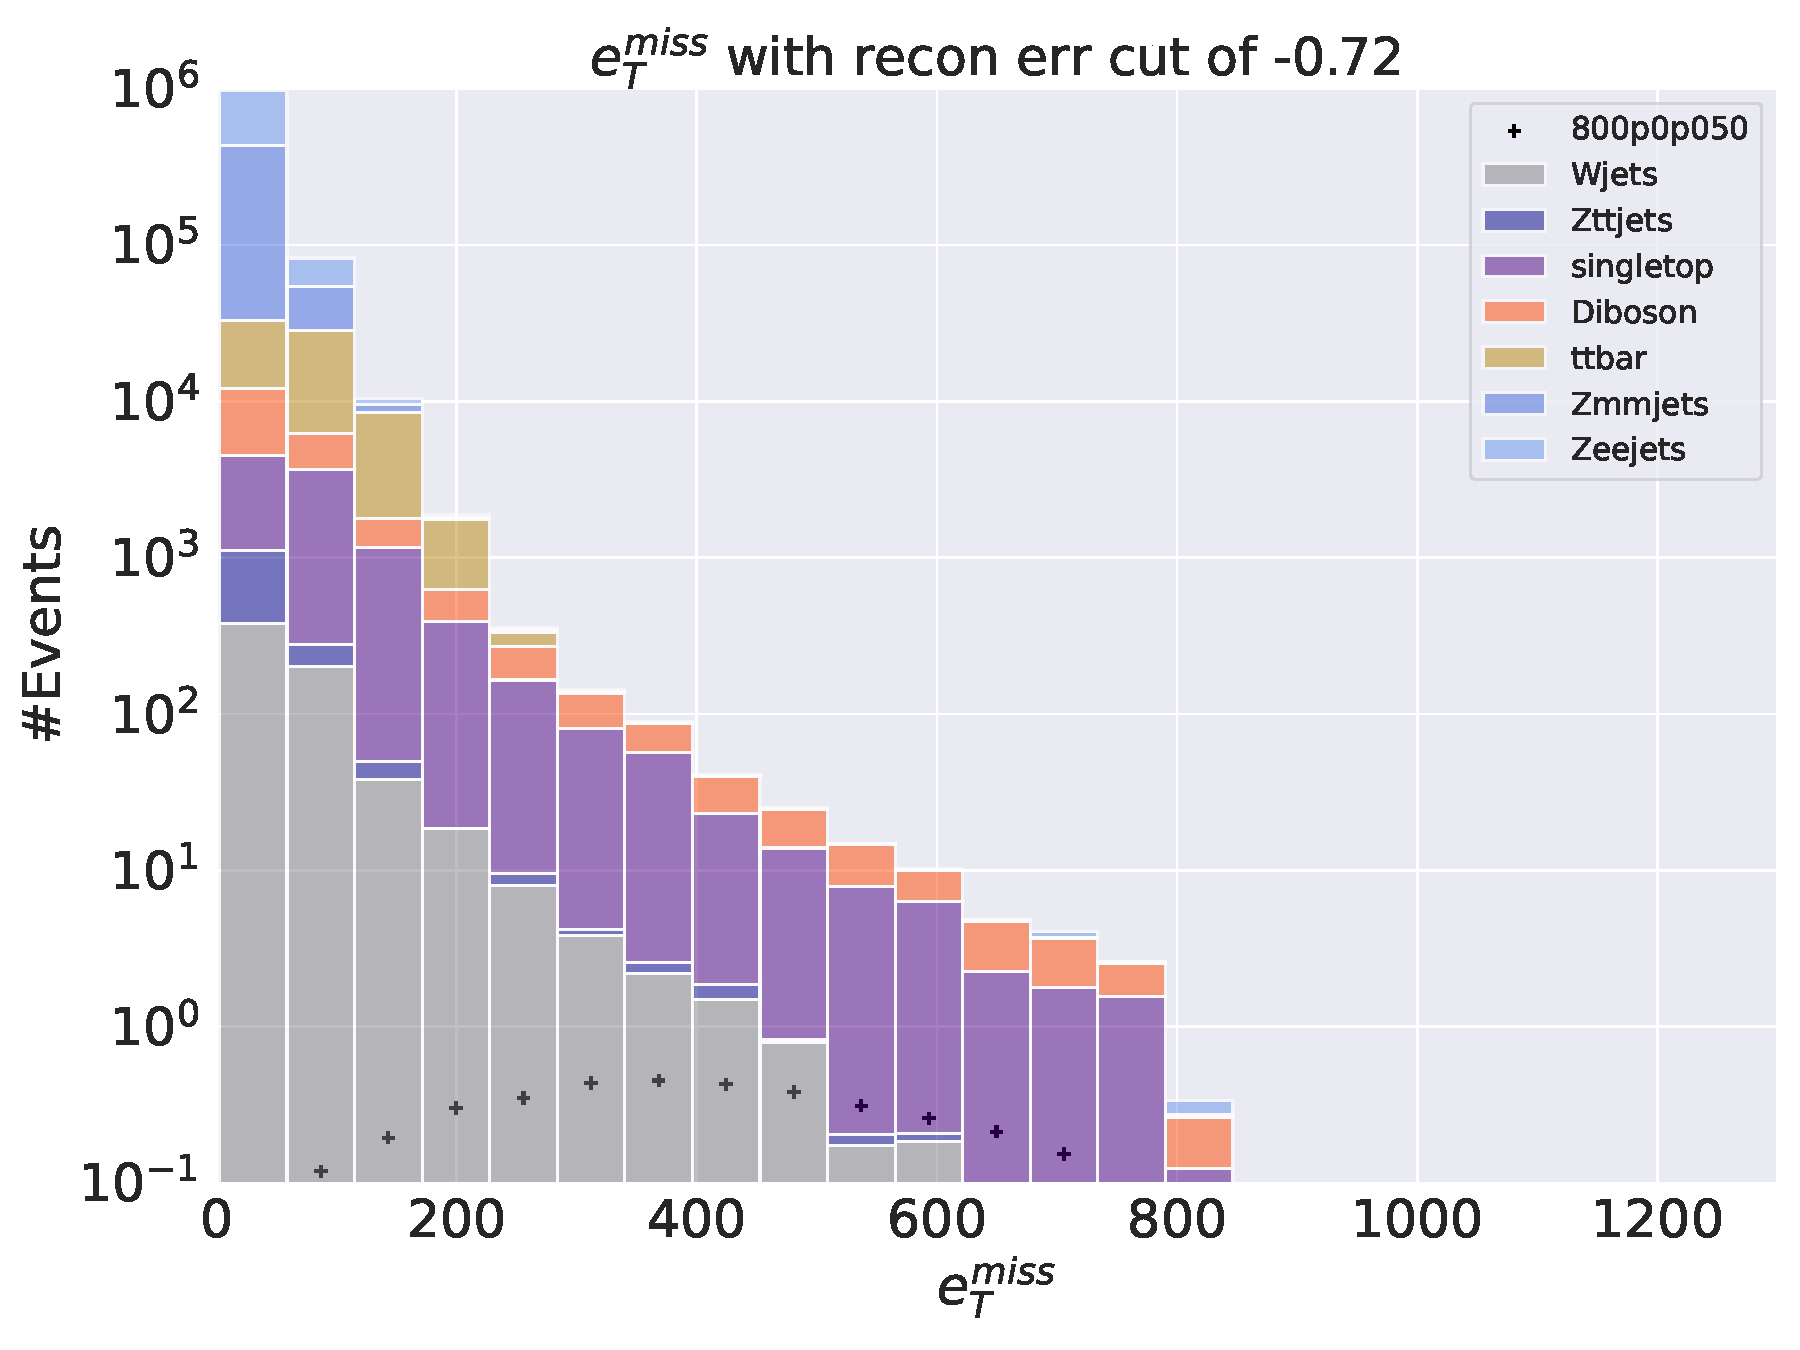
\includegraphics[width=\textwidth]{Figures/VAE_testing/big/2lep/b_data_recon_big_rm3_feats_sig_800p0p050_recon_errcut_-0.72.pdf}
        \caption{}
        \label{fig:VAE_2lep_big_etmiss_800}
    \end{subfigure}
    \hfill
      
    \begin{subfigure}{.49\textwidth}
        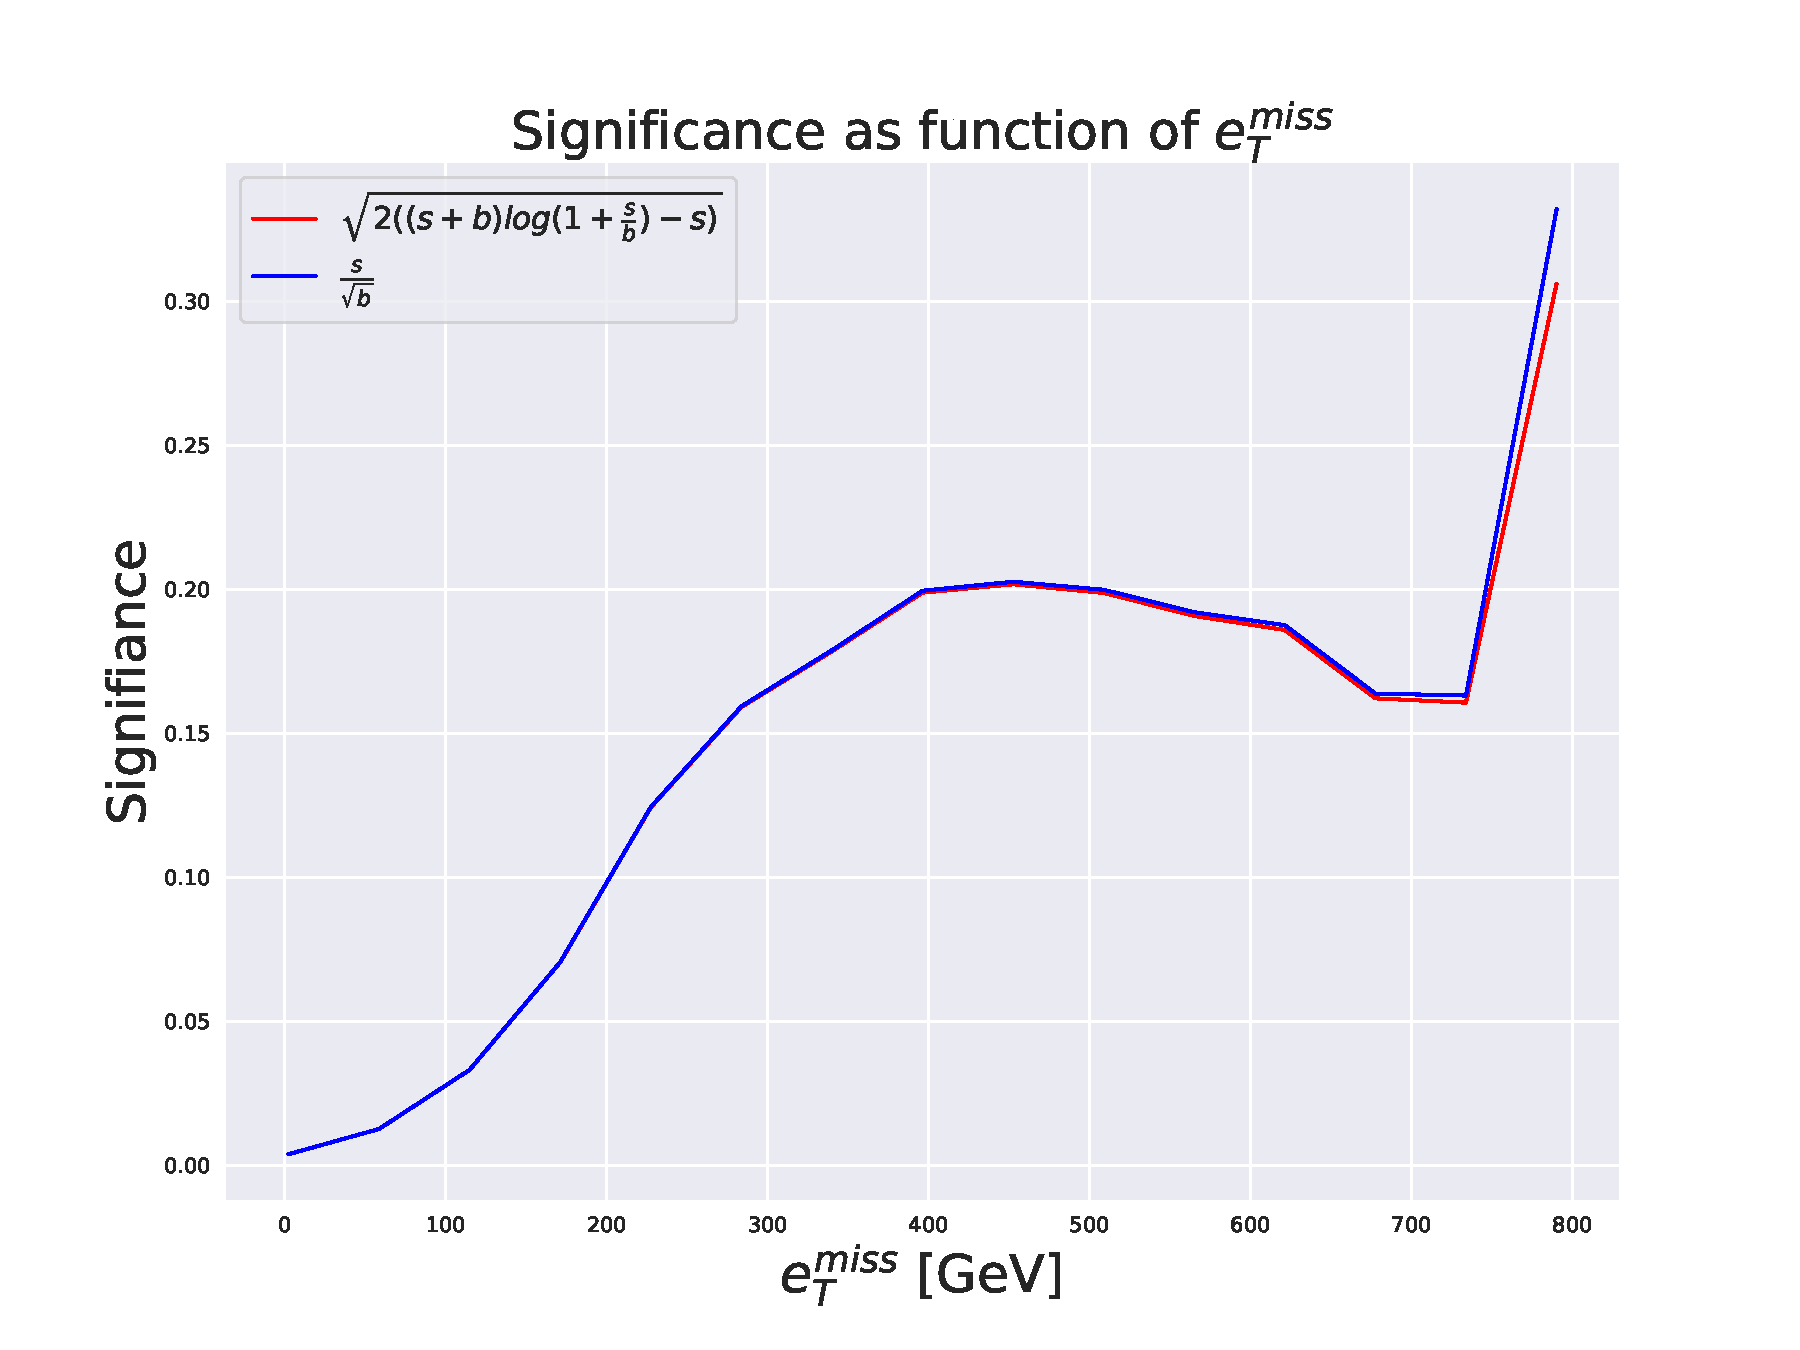
\includegraphics[width=\textwidth]{Figures/VAE_testing/big/2lep/significance_etmiss_800p0p050_-0.7232197345309495.pdf}
        \caption{}
        \label{fig:VAE_2lep_big_signi_800}
    \end{subfigure}
    \hfill      
    \caption[2lep deep network | $800p50$ | VAE]{Reconstruction error (a), $e_T^{miss}$ signal region (b) and significance as function of 
    $e_T^{miss}$ (c) for the deep variational autoencoder using SUSY $800p50$.
    (a) shows that the peak of the distribution is somewhat centered in the middle 
    of the reconstruction error range forming a hill-like shape. The peaks of the background and signal 
    distributions are not well separated, with some separation of distribution peaks. (b) 
    shows a signal region with large background distribution. The signal region is made using a cut around
    $10^{-0.72}$. The peaks in the signal region are also somewhat 
    separated, but the overall distributions are overlapping still. 
    (c) shows the significance as function of $e_T^{miss}$.
The peak significance is around 0.20 at around 450 GeV.}
    \label{fig:VAE_2lep_big_rec_sig_signi_800}
\end{figure}

\begin{figure}[h!]
    \centering
    \begin{subfigure}{.49\textwidth}
        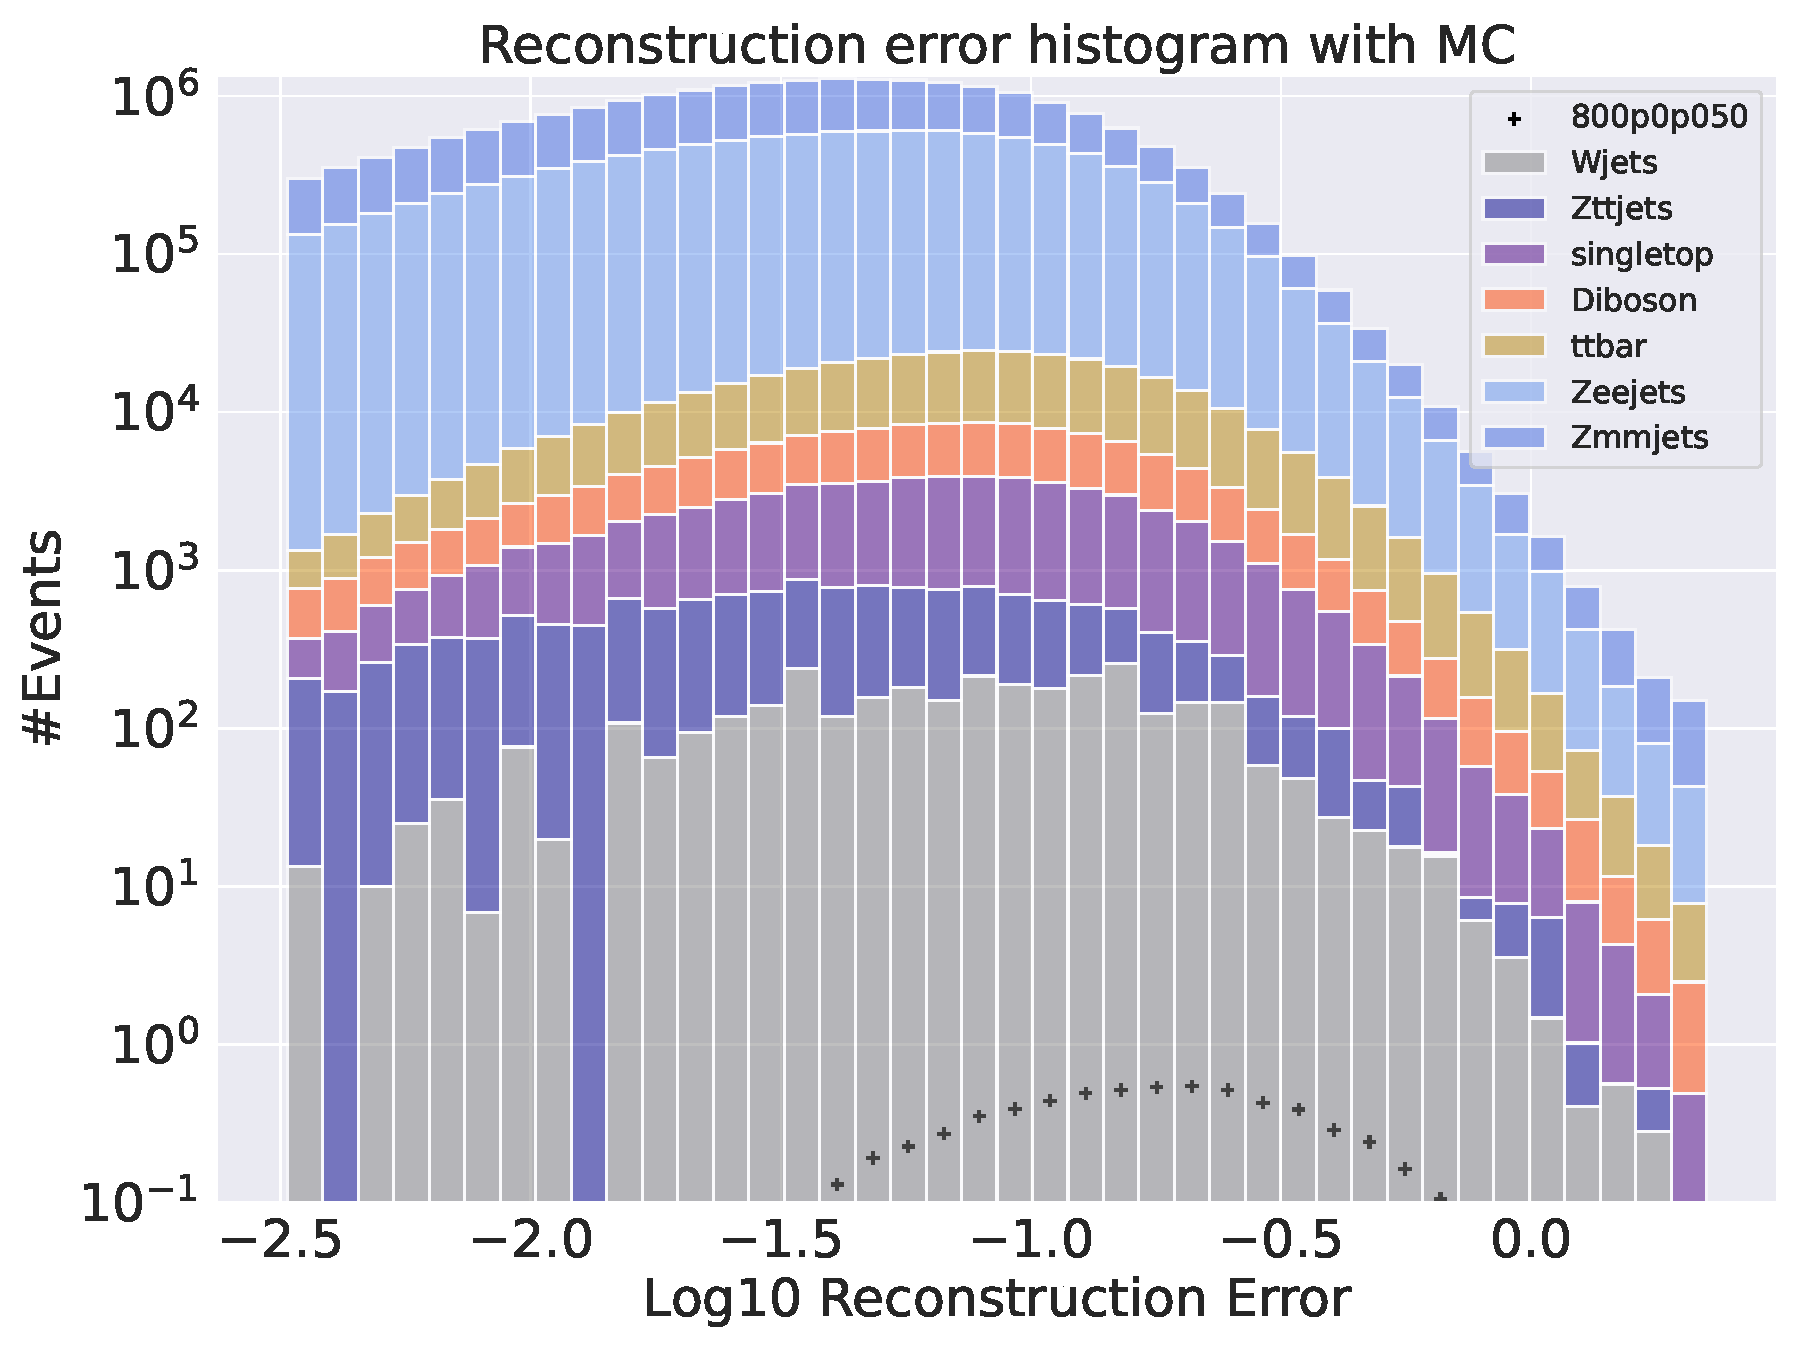
\includegraphics[width=\textwidth]{Figures/VAE_testing/small/2lep/b_data_recon_big_rm3_feats_sig_800p0p050_.pdf}
        \caption{ }
        \label{fig:VAE_2lep_small_800}
    \end{subfigure}
    \hfill
    \begin{subfigure}{.49\textwidth}
        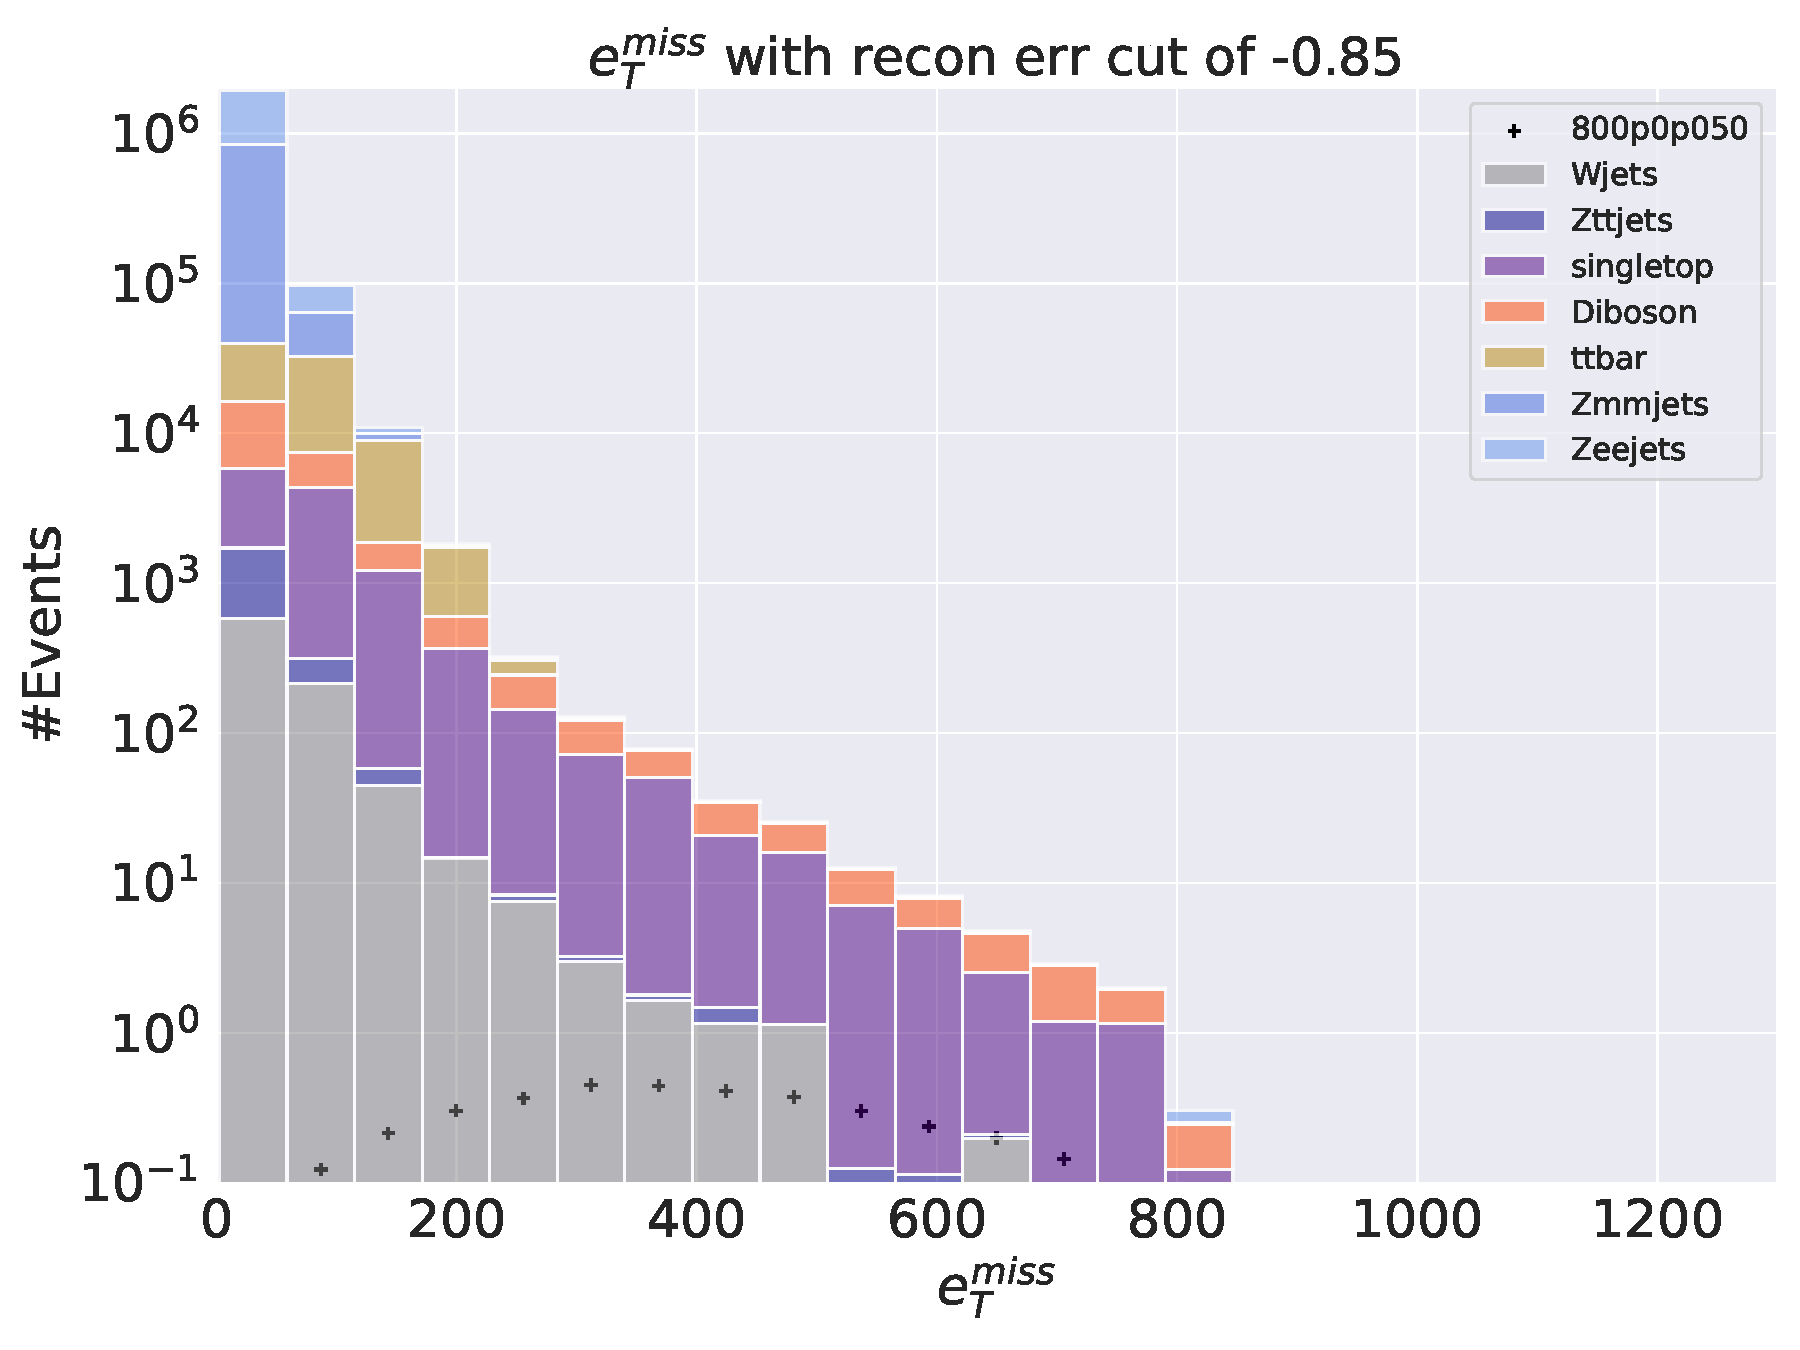
\includegraphics[width=\textwidth]{Figures/VAE_testing/small/2lep/b_data_recon_big_rm3_feats_sig_800p0p050_recon_errcut_-0.85.pdf}
        \caption{}
        \label{fig:VAE_2lep_small_etmiss_800}
    \end{subfigure}
    \hfill  
    \begin{subfigure}{.49\textwidth}
        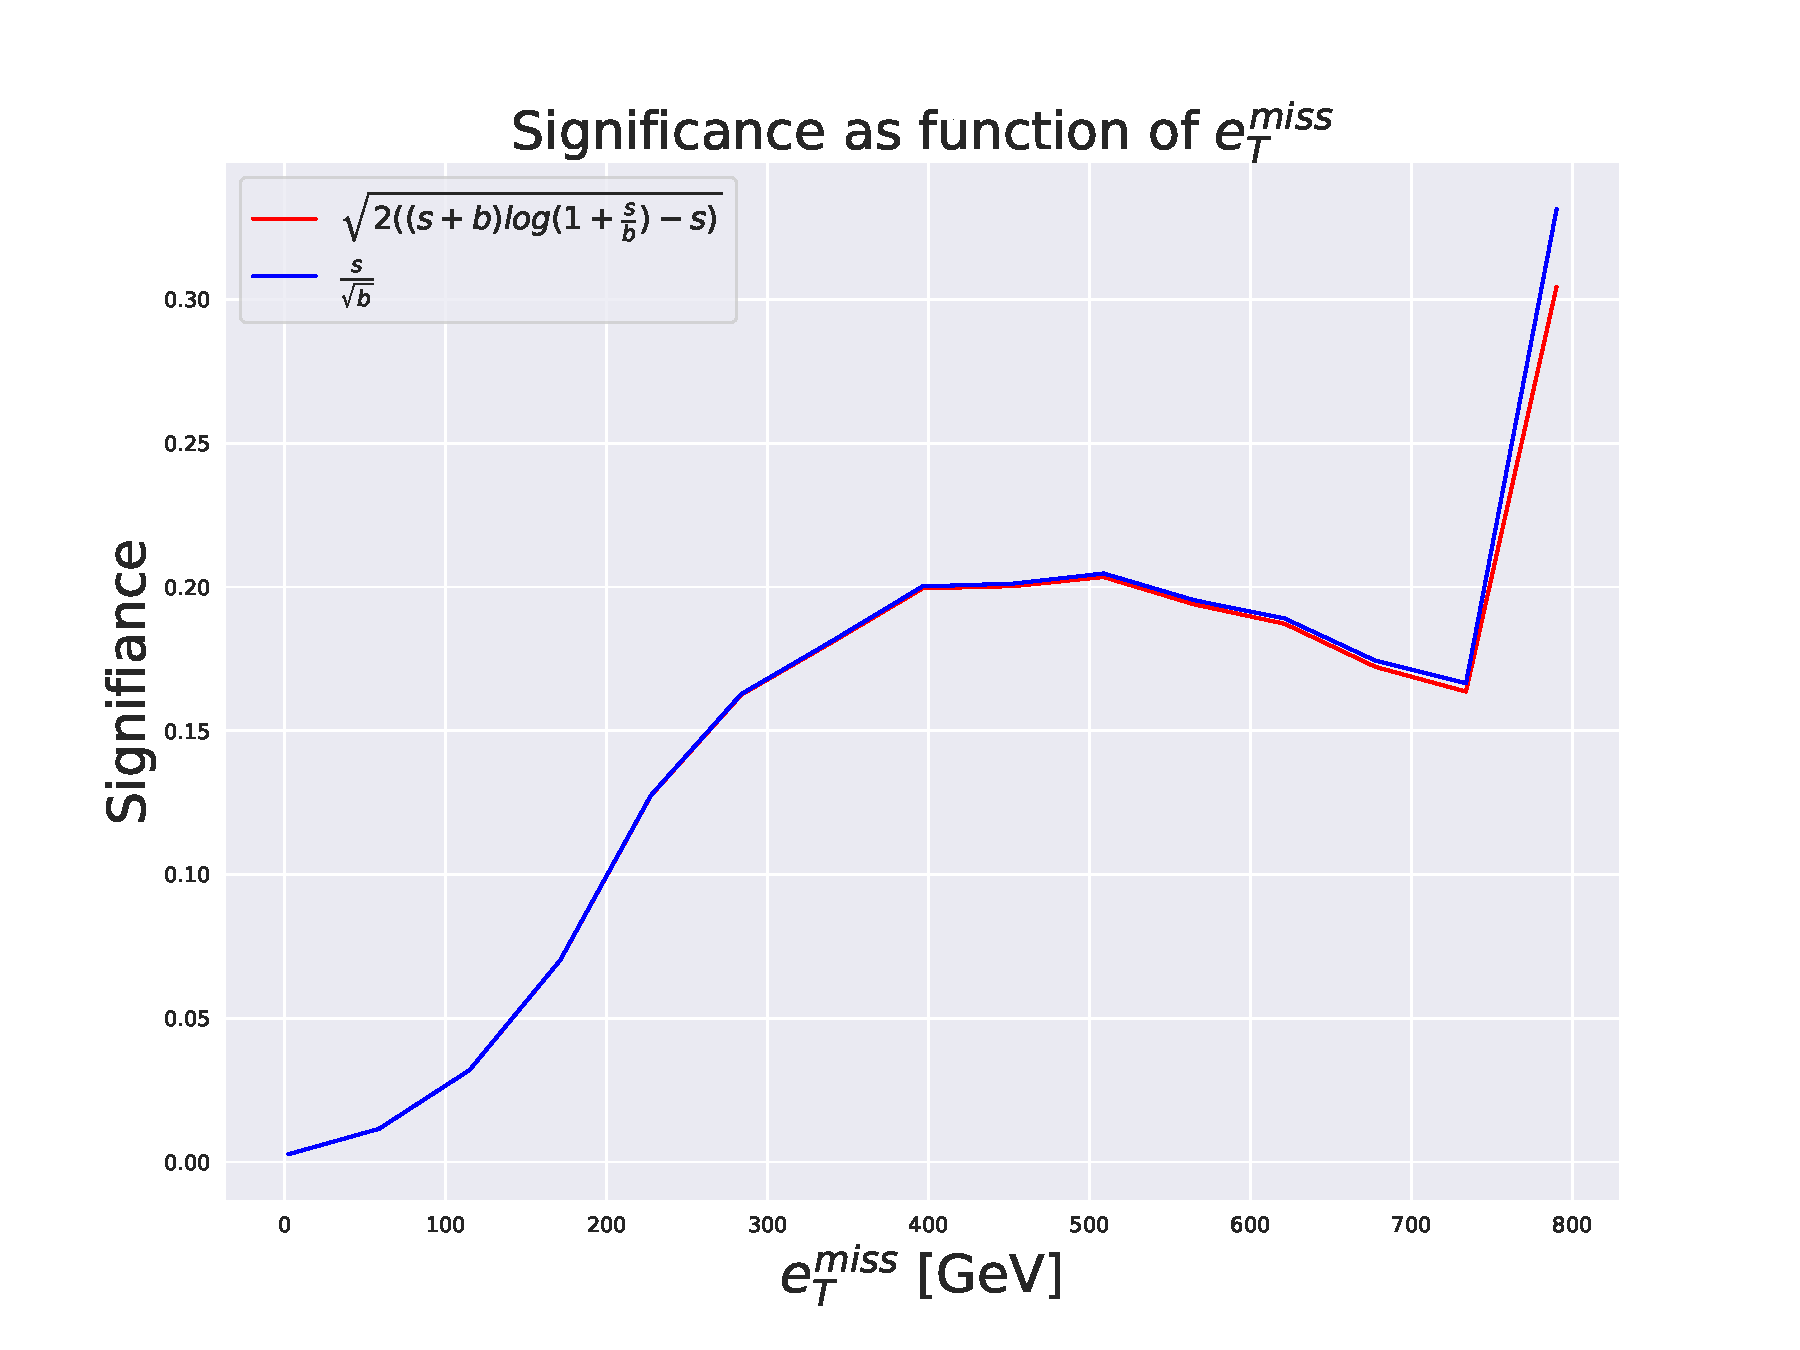
\includegraphics[width=\textwidth]{Figures/VAE_testing/small/2lep/significance_etmiss_800p0p050_-0.8542149600758421.pdf}
        \caption{}
        \label{ffig:VAE_2lep_small_signi_800}
    \end{subfigure}
    \hfill      
    \caption[2lep shallow network | $800p50$ | VAE]{Reconstruction error (a), $e_T^{miss}$ signal region (b) and significance as function of 
    $e_T^{miss}$ (c) for the shallow variational autoencoder using SUSY $800p50$. 
    (a) shows that the peak of the distribution is somewhat centered in the middle 
    of the reconstruction error range forming a hill-like shape. The peaks of the background and signal 
    distributions are not well separated, with almost identical reconstruction error pattern. (b) 
    shows a signal region with large background distribution. The signal region is made using a cut around
    $10^{-0.72}$. The peaks in the signal region are also somewhat 
    separated, but the overall distributions are overlapping still. 
    (c) shows the significance as function of $e_T^{miss}$.}
    \label{fig:VAE_2lep_small_rec_sig_signi_800}
\end{figure}


In figures \ref{fig:VAE_2lep_big_rec_sig_signi_450}, \ref{fig:VAE_2lep_small_rec_sig_signi_450}, 
\ref{fig:VAE_2lep_big_rec_sig_signi_800} and \ref{fig:VAE_2lep_small_rec_sig_signi_800} we have three 
subplots containing the total reconstruction error distributions, the $e_T^{miss}$ signal region, 
and the significance as function of $e_T^{miss}$ curve respectively. They were created using 
the shallow and deep regular autoencoder with the 2 lepton + $e_T^{miss}$ dataset. \par
In figures \ref{fig:VAE_2lep_big_450}, \ref{fig:VAE_2lep_small_450}, \ref{fig:VAE_2lep_big_800}, 
\ref{fig:VAE_2lep_small_800} we have the reconstruction error distributions 
for both SUSY signals for the small and large variational autoencoder. 
The steepness here differs from the steep slope in figures 
\ref{fig:AE_2lep_big_450}, \ref{fig:AE_2lep_small_450}, \ref{fig:AE_2lep_big_800}, 
\ref{fig:AE_2lep_small_800}. Interestingly, we see here that the deepness of the neural 
network here plays a role, which is different from the regular autoencoder output, where both 
the small and large autoencoder made a steep slope shape of the SM MC reconstruction error 
distribution. The peak of the distribution here is slightly shifted to the left for the shallow 
autoencoder model, and slightly shifted to the right of the center with the deep autoencoder 
model. One possible reason for this somewhat hill-like distribution could be that the 
variational autoencoder samples from a Gaussian distribution that has yet to be trained on 
enough data to produce a good enough error distribution. 
% This is also supported with the fact 
% that the shape is even more hill-like like in the 3 lepton + $e_T^{miss}$ case shown in 
% figures \ref{fig:VAE_3lep_big_450}, \ref{fig:VAE_3lep_small_450}, \ref{fig:VAE_3lep_big_800}, 
% \ref{fig:VAE_3lep_small_800}. It could also be that the batch size is too large, and that 
% the model has to train on smaller batches to get a better result. 
\par 

In figures \ref{fig:VAE_2lep_big_etmiss_450}, \ref{fig:VAE_2lep_small_etmiss_450}, 
\ref{fig:VAE_2lep_big_etmiss_800} and  \ref{fig:VAE_2lep_small_etmiss_800} we have 
the $e_T^{miss}$ distribution for the least strict cut for each signal. We see that 
the cuts are somewhat similar to the regular autoencoder, but with two key differences.
First, because the peaks of the distributions from figures \ref{fig:VAE_2lep_big_450}, 
\ref{fig:VAE_2lep_small_450}, \ref{fig:VAE_2lep_big_800}, \ref{fig:VAE_2lep_small_800} 
are so close, the cuts allowed for more background events in the signal region. Here, 
as with the regular autoencoder output, the reconstruction cut from section \ref{sec:strategy} 
$m_{err}$ was used to create the signal region, 
but was not a good descriminator for the background events. Still, because we set 
cuts based on reconstruction error to mimimize the background in the signal region, 
if one does have overlapping distributions with similar slopes, the results will be poor in comparison. \par
Secondly, the background that remains are slightly Although the peak in both
signal models are fairly separated from the peak of the SM MC, the SUSY 800p50 signal model is shifted a
bit more to the right end. The reason for the low signifcance is that the cross-section is much lower for the
different from the signal region from the regular autoencoder. In the lower energy range there 
is a large excess of Zeejets, Zmmjets and ttbar events that have a high reconstruction error, 
which is not the case for the variational autoencoder, dominated by diboson events in all bins. 
In the higher energy range, diboson are largest contributer to the background, but the number 
of bins are exceptionally smaller than the Zmmjets/Zeejets/ttbar events, by a magnitude of 3 at the most. 








